% Neurocomputing submission (Elsevier elsarticle).
% Build: latexmk -pdf main.tex
\documentclass[preprint,12pt]{elsarticle}

\usepackage[T1]{fontenc}
\usepackage[utf8]{inputenc}
\usepackage{amsmath,amssymb,amsthm}
\usepackage{graphicx}
\usepackage{booktabs}
\usepackage{multirow}
\usepackage{siunitx}
\usepackage{algorithm}
\usepackage{algpseudocode}
\usepackage{url}
\usepackage[hidelinks]{hyperref}
\usepackage{cleveref}
\usepackage{tikz}
\usetikzlibrary{positioning,arrows.meta}
\usepackage{xcolor}
\usepackage{lineno}
\usepackage{setspace}

\graphicspath{{../figures/}{figures/}}
\bibliographystyle{elsarticle-num-names}

\newtheorem{proposition}{Proposition}
\newtheorem{corollary}{Corollary}
\newtheorem{theorem}{Theorem}
\newtheorem{lemma}{Lemma}
\theoremstyle{definition}
\newtheorem{definition}{Definition}
\theoremstyle{remark}
\newtheorem{remark}{Remark}

\newcommand{\cD}{\mathcal{D}}
\newcommand{\cR}{\mathcal{R}}
\newcommand{\cS}{\mathcal{S}}
\newcommand{\bE}{\mathbb{E}}
\newcommand{\bR}{\mathbb{R}}
\newcommand{\wh}[1]{\widehat{#1}}

\setlength{\emergencystretch}{2em}

\renewcommand{\topfraction}{0.9}
\renewcommand{\bottomfraction}{0.8}
\renewcommand{\textfraction}{0.07}
\renewcommand{\floatpagefraction}{0.75}

\journal{Neurocomputing}

\begin{document}

\begin{frontmatter}

\title{Stage-conditional shift normalization for subject-robust EEG sleep
staging}

\author[aff1]{Zhiwen Song}
\author[aff1]{Yuhao Peng\corref{cor1}}
\ead{pngyuo@cug.edu.cn}
\cortext[cor1]{Corresponding author. ORCID: 0009-0004-3302-9050.}
\affiliation[aff1]{organization={School of Mathematics and Physics,
            China University of Geosciences (Wuhan)},
            addressline={388 Lumo Road, Hongshan District},
            city={Wuhan},
            postcode={430074},
            country={China}}

\begin{abstract}
Automatic sleep staging models can lose accuracy when applied to unseen
patients, yet a single label-free remedy is usually applied: replace the
normalization statistics of the target recording. This assumes that subject
shift is a recording-wide offset. We introduce a patient-identity diagnostic
that tests this assumption by refitting a linear subject probe within each
sleep stage. After marginal mean correction, the within-stage probe remains
well above chance, whereas the overall probe is dominated by the removable
offset. We therefore propose stage-conditional shift normalization (SCSN), a
closed-form, label-free correction that estimates a separate shift for each
stage from the model's soft posterior and subtracts the posterior-weighted
shift during inference. SCSN contains marginal correction as its $\lambda=0$
endpoint and applies unchanged to batch- and group-normalized networks.
Across Sleep-EDF (39 recordings), HMC (151 recordings), two backbones and two
normalization schemes, SCSN reduced the within-stage subject probe from
$0.74$ to $0.47$ and from $0.53$ to $0.21$ on EEGNet. Classification accuracy
was preserved on Sleep-EDF and improved by $1.4$--$1.9$ points on HMC. On
group-normalized models, SCSN significantly improved accuracy in three of four
settings and improved worst-patient conformal coverage in all four. Cross-cohort
transfer also exposes the method's precondition: a weak target posterior
reduces SCSN to marginal correction, whereas oracle stages recover most of the
gap.

\end{abstract}

\begin{keyword}
Sleep staging \sep Test-time adaptation \sep normalization \sep
Subject variability \sep Electroencephalography \sep Conformal prediction
\end{keyword}

\end{frontmatter}

\ifdefined\REVIEWCOPY
\doublespacing
\linenumbers
\fi

\section{Introduction}
\label{sec:intro}

A deep network trained to stage sleep agrees with a human scorer about as well
as two human scorers agree with each other, provided the patient comes from the
cohort it was trained on. Applied to a patient from another clinic, the same
network loses a substantial part of that agreement. The loss is not a failure
of the filters: a slow oscillation is a slow oscillation in every laboratory.
It is a failure of the statistics with which the network represents the
patient, and those statistics are produced, to a large extent, by the
normalization layers.

The default label-free remedy is marginal adaptation. Re-estimating the
batch-normalization statistics on the recording being scored --- adaptive batch
normalization, AdaBN \citep{li2018adabn} --- removes one mean and one variance
per layer and per night, uses no label and changes no weight. It is cheap,
deterministic and widely used. Its premise is that the patient is a
recording-wide offset. This paper shows that the premise is only half true,
and that the half it misses is the one that a single vector per recording
cannot address.

\paragraph{Two parts of the patient}
The class-conditional mean of the representation in a recording decomposes
exactly into three terms (Section~\ref{sec:method}): the stage prototype
$\mu_k$ the classifier was trained on, a recording-wide offset
$a_{\cR}$ that is the same for every epoch of the night, and a
stage-conditional signature $s_{\cR,k}$ that describes how this patient's
wake, N2 or REM differs from the prototype. The post-hoc mean subtraction
that mimics AdaBN at the representation removes $a_{\cR}$ and leaves
$s_{\cR,k}$ untouched; layerwise AdaBN removes $a_{\cR}$ and, as a nonlinear
side effect, in some settings part of $s_{\cR,k}$, but it has no stage index
and cannot target it. The residual is not small either way. Within each stage a linear probe
still identifies the patient far above chance after layerwise AdaBN, and the
conditional part of the residue is what the classifier compares when it
decides between two stages: the logit margin under a marginal correction is
perturbed by $s_{\cR,j}-s_{\cR,k}$.

\paragraph{Stage-conditional shift normalization}
If the shift is indexed by the stage, it can be removed stage by stage. SCSN
estimates, for each stage $k$ and recording $\cR$, the shift
$\hat\delta_{\cR,k}$ between the recording's stage-conditional mean and the
cohort prototype, and subtracts the posterior-weighted average of those shifts
from every epoch:
$\tilde z_i=z_i-\sum_k p_{ik}\hat\delta_{\cR,k}$, where $p_{ik}$ is the
model's own softmax on the uncorrected representation. The estimator is
closed-form with one shrinkage constant, uses no label, changes no weight, and
needs no additional forward pass: the representation and the posterior come
from the same pass over the night. The offset cancels for any
posterior that sums to one; the stage-conditional signature cancels when the
posterior is informative. Under the population correction the class-conditional
means of every recording are mapped back to $\mu_k$, so the logit margin
between any two stages is restored to the one the head was trained on.
Setting the mixing parameter of the interpolated form to zero recovers the
marginal correction, so the two are endpoints of one family rather than
unrelated methods.

\paragraph{Why the distinction matters in practice}
The distinction is not only analytical. A batch-normalized stager can be
adapted by replacing its statistics, and the test-time adaptation literature
has produced a family of increasingly elaborate ways to do so
\citep{li2018adabn,wang2021tent,cafa2023,unmixtns2024,psdnorm2026}. A
group-normalized stager cannot use the standard AdaBN replacement: its
normalization is computed within an epoch and therefore has no test-time batch
statistic to re-estimate. A bespoke entropy objective on GroupNorm's affine
parameters could be constructed, but this is not the usual Tent procedure and
we treat it as a separate method outside this study. Yet group normalization
is an increasingly common choice precisely because it removes dependence on
batch composition, and the representation it produces still carries the
patient. On these checkpoints we compare the uncorrected model, the post-hoc
marginal correction, and SCSN; SCSN is the only stage-aware method among the
statistics-replacement approaches evaluated here.

The same failure separates SCSN from existing transfer methods for sleep and
EEG. Cross-domain sleep staging has been addressed by test-time adaptation
\citep{guo2025tta}, whereas recent cross-subject models use meta-learning,
domain alignment, or self-supervised representation learning
\citep{metasth2026,sedaeeg2025,transformeeg2026}. These approaches improve
subject generalization by changing training objectives or learned
representations. SCSN leaves both the trained filters and the classifier
unchanged and corrects only recording-level statistics that remain after
training.

\paragraph{Measuring the right quantity}
A subject-identification probe fitted to the penultimate representation is
the natural diagnostic, but the overall probe is dominated by the marginal
component: any per-recording centering collapses it, whether or not the
conditional signature survives. We therefore refit the probe \emph{within
each stage}. The within-stage probe is unchanged by a correction that removes
only $a_{\cR}$, and falls only when the correction removes $s_{\cR,k}$. The
distinction is what separates the two families empirically, and it is the
measurement we report throughout.

\paragraph{What kind of contribution this is}
The contribution is analytical before it is algorithmic. The paper adds no
layer, no loss and no training procedure; it characterizes what a trained
stager's representation contains and which inference-time operations can change
which part of it, and the algorithm follows from that characterization. Two
results carry it. The first is an identity: the class-conditional means of a
recording decompose exactly into a cohort prototype, a recording-wide offset
and a stage-conditional signature, and the two parts are identifiable from each
other by construction. The second is an impossibility statement, which we
prove rather than observe: every correction that subtracts one vector per
recording --- an oracle that knows the patient's stage mix, an estimate of the
recording mean, any vector learned from the recording --- leaves the relative
configuration of the stage-conditional means unchanged
(Corollary~\ref{cor:no-marginal}). No better estimate of the marginal statistic
can remove the signature, because the signature is not a statistic of the
recording's mean; only an operation indexed by the stage can reach it. SCSN is
then derived rather than designed: given the posterior, the posterior-weighted
average of the per-stage shifts is the minimum-mean-square-error estimate of
the shift that affects an epoch, and the residual is the posterior mass placed
on the wrong stage (Remark~\ref{rem:mmse}). That it has a closed form is a
consequence of the setting the method is meant for --- a checkpoint whose
weights are frozen and a night that carries no labels --- and the closed form
is the reason the method is deployable, not the reason it is new. Read as a
normalization operator, SCSN is the class-conditional counterpart of AdaBN: its
sufficient statistics are indexed by the classes the model assigns, rather than
by the batch or by the epoch.

\paragraph{What the paper contributes}
\begin{enumerate}
  \item A decomposition of the penultimate representation into a stage
  prototype, a recording offset and a stage-conditional subject signature,
  with propositions that state exactly what marginal adaptation leaves behind
  (Proposition~\ref{prop:marginal}) and what a stage-conditional correction
  removes (Proposition~\ref{prop:conditional}), and a corollary that no
  correction subtracting one vector per recording can alter the relative
  geometry of the stage-conditional means
  (Corollary~\ref{cor:no-marginal}).
  \item SCSN, a closed-form, label-free normalization of the representation
  that needs no retraining and no optimizer, applies unchanged to
  batch-normalized and group-normalized stagers, and contains the marginal
  correction as the endpoint $\lambda=0$ of a one-parameter family
  (Algorithm~\ref{alg:scsn}).
  \item A measurement protocol that separates the two components of patient
  identity, and evidence on two cohorts, two backbones and two normalization
  regimes that layerwise AdaBN leaves a large within-stage signature while
  SCSN removes several times more of it.
  \item Evidence that on group-normalized stagers, where the standard AdaBN
  statistics replacement is undefined, SCSN remains applicable and removes
  the conditional signature; it also improves accuracy and per-patient
  conformal-coverage dispersion over the uncorrected model.
  \item Controls that isolate the mechanism --- mismatched statistics,
  orthogonalised corrections, hard pseudo-labels, low-rank restrictions ---
  a Tent baseline evaluated on the same runs, and a cross-cohort experiment
  that delimits the regime in which a stage-conditional correction is useful.
\end{enumerate}

The method is offline in the same sense as AdaBN: it reads the unlabeled
epochs of the night it is about to score. Clinical staging is performed after
the night, so this is the setting in which a deployed stager operates. No
label, no epoch of another patient and no weight is used.

The paper reports where the method is not the best available one. On
Sleep-EDF SleepCNN, layerwise AdaBN is $1.4$ points more accurate than SCSN,
a difference that is not significant; on Sleep-EDF EEGNet the two are
indistinguishable; and Tent is competitive on the same cohort. On both HMC
backbones SCSN has the highest mean accuracy of the arms, by a margin that is
significant over the uncorrected model in both cases and not significant over
layerwise AdaBN on HMC SleepCNN. The claim defended here is not that
SCSN dominates every baseline on accuracy, but that it removes a component of
patient identity that none of them removes, and that this component can be
measured, predicted and corrected without labels.

\paragraph{Organisation}
Section~\ref{sec:related} places the work among test-time normalization and
subject-variability methods. Section~\ref{sec:method} derives the
decomposition, states the propositions and defines the algorithm.
Section~\ref{sec:setup} describes the cohorts, arms, metrics and statistics.
Section~\ref{sec:results} reports the main comparison, the mechanism analyses,
the ablations, the Tent baseline, the group-normalized setting and
cross-cohort transfer. Section~\ref{sec:discussion} discusses what the results
do and do not license.

\section{Related work}
\label{sec:related}

\subsection{Normalization as a statistical interface}

Batch normalization \citep{ioffe2015bn} is usually discussed for what it does
during training. At inference it is a different object: a fixed affine map
whose slope and offset were estimated on the training cohort, so that the
representation of a test recording carries a term determined by how far that
recording's statistics lie from the cohort's. Group normalization
\citep{wu2018group}, instance normalization \citep{ulyanov2016instance} and
layer normalization \citep{ba2016layer} remove the batch from the computation
and make the output of the layer depend only on the example it is applied to.
\citet{frankle2021bn} show how much of a trained network's function is
reproduced by its normalization parameters alone, and \citet{nado2020}
evaluate prediction-time batch normalization under covariate shift; both
locate a large part of the model's behavior in statistics rather than in
filters.

Re-estimating the statistics on the test domain is adaptive batch
normalization \citep{li2018adabn}. In sleep staging the operation is
attractive because a night is a natural adaptation domain: its epochs are
exchangeable enough to estimate a mean and variance, and no label is needed.
What the operation cannot do is distinguish one sleep stage from another. It
estimates one mean per recording, so any patient-dependent component that
differs between stages survives it. This is the gap the present paper
addresses.

A related line conditions normalization on a label. Conditional batch
normalization and feature-wise transformations modulate the activations of a
network with a class or text embedding
\citep{devries2017modulating,dumoulin2018feature,perez2018film}; the
conditioning signal is known during training and supplied at inference. SCSN
conditions on the stage as well, but it does not learn a conditioning map and
it does not receive the stage: the stage is unknown at test time and is
replaced by the model's own soft posterior. The weights stay frozen, and the
only quantity estimated from the test recording is the shift itself.

The ingredients of the method are ordinary --- estimate a mean, subtract it,
index the estimate by a class --- so the question is what the paper contributes
beyond their assembly. The answer is the result that links them. The
decomposition of Section~\ref{sec:method} proves that no correction subtracting
one vector per recording can change the relative configuration of the
stage-conditional means, however well that vector is estimated
(Corollary~\ref{cor:no-marginal}); feature-wise modulation, in turn, is
supplied with a class taken from an annotation, whereas in staging the class is
unknown and the index has to be estimated from the model.
The two observations only become one contribution when the first shows that the
marginal route cannot work and the second shows what has to replace it. SCSN is
the normalizer that results: class-conditional statistics, conditioned on a
test-time estimate of the class rather than on a label. The experiments test
the derivation rather than a combination --- the interpolation between the
marginal and conditional endpoints, the matched-versus-mismatched control, and
the cross-cohort test in which a weak posterior should and does reduce the
method to its marginal special case.

\subsection{Test-time adaptation beyond marginal statistics}

Tent \citep{wang2021tent} updates the affine parameters of normalization
layers by minimizing the entropy of the posterior on the test recording;
test-time training \citep{sun2020ttt} uses a self-supervised objective. Both
change weights with an optimizer. CAFA \citep{cafa2023} aligns target features
to the source distribution with a class-aware objective, and UnMix-TNS
\citep{unmixtns2024} improves the estimation of normalization statistics when
test labels are temporally correlated. PSDNorm \citep{psdnorm2026} replaces
mean-and-variance normalization by a test-time alignment of the power spectral
density of each feature map and reports strong cross-dataset sleep staging;
the operation is input-domain and frequency-resolved, and it does not use the
predicted stage. FairAdaBN \citep{fairadabn2023} makes adaptive normalization
attribute-aware for fairness.

SCSN differs from this family in three respects. It is closed-form: no
optimizer, step size or number of steps is chosen at test time. It is
stage-conditional: the statistic it removes is indexed by the sleep stage, and
the index comes from the model's own posterior rather than from a label or a
frequency band. And its target is explicit: the class-conditional mean of the
representation, which is the quantity the classifier's decision boundaries were
fitted around. The interpolated form in Section~\ref{sec:method} contains the
post-hoc marginal correction as the endpoint $\lambda=0$, so the comparison is
a nested one rather than a comparison of unrelated methods.
Cross-domain sleep staging has also been addressed directly by test-time
adaptation \citep{guo2025tta}. The distinction from SCSN is the conditioning
variable: these methods adapt a shared target-domain or test-domain
transformation, whereas SCSN updates a separate first-moment correction for
each posterior-indexed sleep stage before the shared classifier is applied.

The family also has a blind spot that matters for the present paper. AdaBN,
Tent and their descendants operate on batch-normalization statistics or
affine normalization parameters. A group-normalized stager has no batch
statistic to replace; a bespoke entropy objective on its affine parameters
would be a different method from standard Tent and is not evaluated here.
Group normalization is an increasingly common choice precisely because it
removes dependence on batch composition, so the lack of a comparable
statistics-replacement correction is a practical gap. SCSN is defined on the
representation and therefore applies unchanged. The other correction compared
for such a checkpoint is post-hoc centering, which
removes one vector per recording; the experiments show that this removes the
overall subject probe while moving the within-stage probe by no more than a
third of what SCSN removes.

\subsection{Subject variability in automatic sleep staging}

Deep stagers have moved from single-cohort evaluation
\citep{supratak2017,phan2019seqsleepnet} to multi-cohort and cross-cohort
settings \citep{perslev2021,phan2022sleepformer}, and the gap between
within-cohort and cross-cohort accuracy has become an object of study.
\citet{nasiri2021subgrouping} show that population subgrouping improves staging
for under-represented patients. Adversarial subject classifiers
\citep{liao2020trifeaturenet} and disentangled architectures
\citep{s3dnet2026} change the weights so that the representation carries less
of the subject; both require retraining and, in the disentangled case, a
subject-invariance objective. \citet{cross2026} use subject-aware batch
normalization during training for cross-subject brain decoding. Normalization
has also been used as a cross-subject alignment device for EEG
\citep{katthi2021cca}, usually on the raw signal rather than inside the
network.
Recent Neurocomputing studies target subject generalization through few-shot
meta-learning \citep{metasth2026}, semi-supervised domain adaptation
\citep{sedaeeg2025}, and generalizable representation learning for EEG
\citep{transformeeg2026}. Like the methods above, these approaches alter
training or the learned representation; the inference-time decomposition
studied here is complementary and can be applied to their frozen outputs.

These methods answer the question \emph{how do we train a model that does not
encode the subject}. The present paper answers a different question: given a
model that already encodes the subject, which part of the encoding is
removable at inference, and which part is not. The answer separates a
recording-wide offset from a stage-conditional signature; the first is removed
by marginal adaptation and the second by SCSN, and only the second requires a
stage posterior. A disentangled architecture can be combined with SCSN, and we
test SCSN on group-normalized checkpoints for exactly that reason.

\subsection{Uncertainty and patient-level reliability}

Sleep staging is scored with a set of stages, and disagreement on boundary
epochs is documented \citep{rosenberg2013}. Calibration measures whether a
predicted probability means what it says \citep{guo2017}; conformal prediction
produces a set with a finite-sample coverage guarantee
\citep{vovk2005,angelopoulos2023gentle}. Adaptive and regularized scores
tighten the sets \citep{romano2020,angelopoulos2021raps}, and the guarantee has
been extended to time series and distribution drift
\citep{gibbs2021,stankeviciute2021}.

The guarantee is marginal over the exchangeable unit. When the unit is the
patient, a stager can honour it on average while under-covering particular
patients, and a representation that separates patients concentrates the
failures. We therefore report per-patient coverage, its dispersion and the
worst-covered patient, and we ask whether the correction that removes the
patient signature also equalises the coverage. The question is not whether the
guarantee is restored --- it remains marginal --- but whether the mechanism
that concentrates the failures is the mechanism that carries the patient.

\section{Stage-conditional shift normalization}
\label{sec:method}

\subsection{What the normalization layer leaves in the representation}

Let $z_i\in\bR^d$ be the penultimate representation of epoch $i$, let
$k_i\in\{1,\dots,K\}$ be its sleep stage, and let $r(i)$ be the recording it
belongs to. Write $\cR$ for a recording and $\pi_{\cR,k}$ for the fraction of
its epochs scored as stage $k$. The class-conditional mean of the
representation in a recording is
\begin{equation}
  m_{\cR,k} \;=\; \bE\!\left[z_i \mid r(i)=\cR,\, k_i=k\right],
  \qquad
  m_{\cR} \;=\; \sum_{k}\pi_{\cR,k}\,m_{\cR,k},
  \label{eq:means}
\end{equation}
and the cohort mean is $\mu_{\mathrm{coh}}=\sum_k \pi_k \mu_k$, with $\mu_k$ the
class mean over the training cohort and $\pi_k$ its stage mix.

The decomposition that organises the paper is a definition, not an
assumption. Set
\begin{equation}
  a_{\cR} \;=\; m_{\cR}-\bar\mu_{\cR},
  \qquad
  s_{\cR,k} \;=\; m_{\cR,k}-\mu_k-a_{\cR},
  \qquad
  \bar\mu_{\cR}=\sum_k \pi_{\cR,k}\mu_k .
  \label{eq:decomp}
\end{equation}
Then $m_{\cR,k}=\mu_k+a_{\cR}+s_{\cR,k}$ and, by construction,
$\sum_k \pi_{\cR,k}s_{\cR,k}=0$. The three terms have different meanings.
$\mu_k$ is the stage prototype the classifier was trained on. $a_{\cR}$ is a
recording-wide offset: it is the same vector for every epoch of the night and
is what a batch-normalization layer manufactures when the recording's first
and second moments differ from the cohort's. $s_{\cR,k}$ is the part of the
patient that is not an offset: within a stage, this patient's spindles, slow
waves or alpha differ from the cohort prototype in a way that is stable across
the night. The constraint makes the offset and the conditional signature
identifiable from each other.

\subsection{Marginal adaptation removes the offset and keeps the signature}

The default label-free remedy is to replace the cohort statistics by the
recording's, either by re-estimating every batch-normalization statistic
(AdaBN) or, at the representation, by subtracting the recording's mean shift
$m_{\cR}-\mu_{\mathrm{coh}}$. The next proposition states exactly what that
leaves behind.

\begin{proposition}[Marginal residual]
\label{prop:marginal}
Under the decomposition \eqref{eq:decomp}, marginal correction
$z_i\mapsto z_i-(m_{\cR}-\mu_{\mathrm{coh}})$ gives
\begin{equation}
  \bE\!\left[z_i-(m_{\cR}-\mu_{\mathrm{coh}})\mid r(i)=\cR,k_i=k\right]
  \;=\;\mu_k+s_{\cR,k}+\bigl(\mu_{\mathrm{coh}}-\bar\mu_{\cR}\bigr).
  \label{eq:marginal-residual}
\end{equation}
\end{proposition}
\begin{proof}
Substitute $m_{\cR}=\bar\mu_{\cR}+a_{\cR}$ from \eqref{eq:decomp} into the
conditional mean $m_{\cR,k}=\mu_k+a_{\cR}+s_{\cR,k}$ and cancel $a_{\cR}$.
\end{proof}

Two consequences follow. The conditional signature $s_{\cR,k}$ survives
untouched: marginal adaptation removes a vector that is constant across stages
and cannot remove one that is not. And the correction adds
$\mu_{\mathrm{coh}}-\bar\mu_{\cR}$, which is zero only when the recording's
stage mix equals the cohort's. A recording with an atypical architecture
therefore keeps a residual offset that is a function of \emph{how it slept},
not of who the patient is. Even an oracle marginal correction that knows
$\bar\mu_{\cR}$ and subtracts $m_{\cR}-\bar\mu_{\cR}$ would leave
$\mu_k+s_{\cR,k}$; the conditional signature is out of reach of any operation
that uses one mean per recording. The next corollary states that this is not a
property of a particular estimate of the mean but of the entire family.

\begin{corollary}[No single-vector correction removes the signature]
\label{cor:no-marginal}
Let $g$ be any function of the recording alone, and apply the correction
$z_i\mapsto z_i-g(\cR)$. Then for any two stages $j,k$,
\begin{equation}
\begin{aligned}
  &\bE\!\left[z_i-g(\cR)\mid r(i)=\cR,k_i=j\right] \\
  &\quad-\bE\!\left[z_i-g(\cR)\mid r(i)=\cR,k_i=k\right]
  =(\mu_j-\mu_k)+(s_{\cR,j}-s_{\cR,k}),
\end{aligned}
  \label{eq:invariant}
\end{equation}
independently of $g$.
\end{corollary}
\begin{proof}
The same vector $g(\cR)$ is subtracted from both conditional means, and
$m_{\cR,j}-m_{\cR,k}=(\mu_j-\mu_k)+(s_{\cR,j}-s_{\cR,k})$ by
\eqref{eq:decomp}.
\end{proof}

The corollary is the precise sense in which the signature is out of reach of
the marginal family. Whatever $g$ is --- the recording mean, an oracle that
knows the patient's stage mix, or a vector learned from the recording --- the
displacement the head compares between two stages changes by the same
$s_{\cR,j}-s_{\cR,k}$. A better estimate of the marginal statistic moves the
offset and leaves the relative geometry exactly where it was; only an operation
whose index depends on $k$ can change \eqref{eq:invariant}. The statement is a
consequence of the definition rather than of a modeling assumption: the
conditional means are what they are, and the difference between two of them
contains $s_{\cR,j}-s_{\cR,k}$ exactly. What the corollary rules out is
therefore not a particular estimator but a class of interventions.

The consequence for the classifier is equally direct. The logit margin
between two stages under marginal correction is
\begin{equation}
  W\!\left(m'_{\cR,j}-m'_{\cR,k}\right)
  = W\!\left(\mu_j-\mu_k+s_{\cR,j}-s_{\cR,k}\right),
  \label{eq:marginal-margin}
\end{equation}
so the patient's stage-conditional signature is added to the very quantity
the classifier compares. When that signature is large --- an atypical patient,
a recording with unusual stage-specific morphology --- the margin can move
across the decision boundary, and accuracy falls. This is the mechanism behind
the accuracy difference between the marginal and conditional corrections in
Section~\ref{sec:scsn-identity}.

\subsection{Stage-conditional shift normalization}

The alternative is to estimate the shift separately for each stage and to
remove it with the model's own soft assignments. Let
$p_{ik}=\Pr(k_i=k\mid z_i)$ be the posterior of the unadapted model, and let
\begin{equation}
  \hat m_{\cR,k}
  =\frac{\sum_{i:r(i)=\cR}p_{ik}z_i+\lambda_s\mu_k}
         {\sum_{i:r(i)=\cR}p_{ik}+\lambda_s},
  \qquad
  \hat\delta_{\cR,k}=\hat m_{\cR,k}-\mu_k ,
  \label{eq:estimator}
\end{equation}
where $\lambda_s\ge0$ is a pseudo-count that shrinks rare stages towards the
cohort prototype; in all experiments $\lambda_s=10$. The corrected
representation is
\begin{equation}
  \tilde z_i \;=\; z_i-\sum_{k}p_{ik}\,\hat\delta_{\cR,k}.
  \label{eq:scsn}
\end{equation}
Equations \eqref{eq:estimator}--\eqref{eq:scsn} are stage-conditional shift
normalization (SCSN). The operation is a closed-form post-processing of one
forward pass: the pass gives $p_{ik}$ and $z_i$, the per-stage shifts are
accumulated, and the corrected representation is obtained by subtracting the
weighted shifts. No second pass over the network is required. No weight is
updated, no optimizer is run, no label of the recording is read, and no
subject identifier is used.

Read as a normalization operator, \eqref{eq:scsn} has the same shape as the
normalizers reviewed in Section~\ref{sec:related} but different sufficient
statistics: batch normalization uses the moments of a batch, group
normalization the moments of an epoch, and SCSN the class-conditional means of
the recording, weighted by the model's posterior. It is a normalization whose
statistics are indexed by the classes the model assigns.

For a recording of $n$ epochs and penultimate dimension $d$, accumulating the
stage summaries takes $O(nKd)$ arithmetic and $O(Kd)$ additional storage; the
correction has the same arithmetic complexity. No network replay, backward
pass, or gradient is required.

\begin{proposition}[Conditional residual]
\label{prop:conditional}
Let $\hat\delta_{\cR,k}=\delta_{\cR,k}=a_{\cR}+s_{\cR,k}$ (the population
value). Then for every epoch,
\begin{equation}
  \tilde z_i
  = z_i-\sum_k p_{ik}\bigl(a_{\cR}+s_{\cR,k}\bigr)
  = z_i-a_{\cR}-\sum_k p_{ik}s_{\cR,k} .
  \label{eq:cond-exact}
\end{equation}
In particular the offset cancels for \emph{any} posterior with
$\sum_k p_{ik}=1$, and if $p_{ik}=\mathbb{1}[k_i=k]$ the conditional mean of
$\tilde z_i$ is exactly $\mu_k$.
\end{proposition}
\begin{proof}
$\sum_k p_{ik}=1$ gives $\sum_k p_{ik}a_{\cR}=a_{\cR}$. For hard assignments
$\sum_k p_{ik}s_{\cR,k}=s_{\cR,k_i}$, and $\mu_k+a_{\cR}+s_{\cR,k}-a_{\cR}
-s_{\cR,k}=\mu_k$.
\end{proof}

For a soft posterior the residual is
\begin{equation}
  \bE[\tilde z_i\mid r(i)=\cR,k_i=k]
  =\mu_k+\sum_j\bigl(\mathbb{1}[j=k]-p_{ij}\bigr)s_{\cR,j},
  \label{eq:soft-residual}
\end{equation}
so the error is the part of the conditional signature assigned to the wrong
stage. It vanishes when the posterior is correct and is bounded by
$\max_j\|s_{\cR,j}\|\sum_j|\mathbb{1}[j=k]-p_{ij}|$. This is why the method is
robust to an imperfect but informative posterior and why it degrades when the
posterior is close to uniform, a prediction we test in the cross-cohort
experiment.

\begin{remark}[Why the posterior-weighted average]
\label{rem:mmse}
Condition on the recording and write $\Delta_i=a_{\cR}+s_{\cR,k_i}$ for the
shift that affects epoch $i$. Given $z_i$, the least-mean-square estimate of
$\Delta_i$ among functions of $z_i$ is the conditional expectation
\begin{equation}
  \bE[\Delta_i\mid z_i]=a_{\cR}+\sum_k \Pr(k_i=k\mid z_i)\,s_{\cR,k},
  \label{eq:mmse}
\end{equation}
and \eqref{eq:scsn} subtracts this quantity with the model's posterior in place
of the unknown true one. The correction is therefore not a heuristic blend: it
is the estimate that minimizes the expected squared residual, and the residual
it leaves, \eqref{eq:soft-residual}, is the part of the shift attributed to the
wrong stage. The hard-assignment variant replaces the posterior by a point mass;
it has a smaller conditional bias and a larger variance, and the experiments
show that it over-corrects. The interpolated family
$z_i-\delta_{\cR}-\lambda(\sum_k p_{ik}\hat\delta_{\cR,k}-\delta_{\cR})$
traces a path from ignoring the stage ($\lambda=0$) to trusting the posterior
completely ($\lambda=1$).
\end{remark}

The class geometry is preserved by the same argument. Under the population
correction the class-conditional means of the corrected representation are
$\mu_k$, independently of the recording, so
\begin{equation}
  W\!\left(\tilde m_{\cR,j}-\tilde m_{\cR,k}\right)
  = W\!\left(\mu_j-\mu_k\right)
  \label{eq:scsn-margin}
\end{equation}
for every recording: the logit margin the classifier was trained on is
restored, whereas under marginal correction it is perturbed by
$s_{\cR,j}-s_{\cR,k}$ as in \eqref{eq:marginal-margin}. This is the formal
content of the accuracy result: SCSN does not merely remove a nuisance, it
maps every recording back to the class geometry on which the head was fitted.

Two controls follow from the algebra. If the correction is constrained to the
null space of $W$, the logits are unchanged exactly, so any change in identity
cannot be attributed to a change in predictions; we implement this by
projecting each $\hat\delta_{\cR,k}$ off the row space of $W$. If the shifts of
a \emph{different} recording are applied, the correction is a non-zero
recording-specific vector and the identity is replaced rather than removed;
this is the matched-versus-mismatched control.

\begin{remark}[Estimation error]
With $n_{\cR,k}=\sum_i p_{ik}$ effective epochs, the shrunk estimator
\eqref{eq:estimator} has bias at most
$\lambda_s\|m_{\cR,k}-\mu_k\|/(n_{\cR,k}+\lambda_s)$ towards the cohort
prototype and standard deviation of order $\|s_{\cR,k}\|/\sqrt{n_{\cR,k}}$.
Both terms are small for the stages that dominate a night (N2, REM) and large
for N1, which is why the shrinkage is kept in all experiments. On HMC a
recording averages about 900 epochs, of which roughly 100 are scored N1 and
330 N2, so a pseudo-count of ten moves the N1 estimate by at most a tenth
towards the prototype and the N2 estimate by at most a thirtieth. The estimator
is a soft, regularized version of the stage-conditional sample mean; no
gradient, iteration or held-out label enters it.
\end{remark}

\begin{algorithm}[t]
\caption{Stage-conditional shift normalization (one recording)}
\label{alg:scsn}
\begin{algorithmic}[1]
\Require frozen stager $f=W\phi+b$, unlabeled epochs $x_1,\dots,x_n$ of a recording $\cR$
\Require cohort class means $\mu_k$ and cohort mean $\mu_{\mathrm{coh}}$
\State $z_i\gets\phi(x_i)$ \Comment{forward pass}
\State $p_{ik}\gets\mathrm{softmax}(Wz_i+b)$
\For{$k=1,\dots,K$}
  \State $\hat m_{\cR,k}\gets(\sum_i p_{ik}z_i+\lambda_s\mu_k)/(\sum_i p_{ik}+\lambda_s)$
  \State $\hat\delta_{\cR,k}\gets\hat m_{\cR,k}-\mu_k$
\EndFor
\State $\tilde z_i\gets z_i-\sum_k p_{ik}\hat\delta_{\cR,k}$ \Comment{correction}
\State \Return $\mathrm{softmax}(W\tilde z_i+b)$
\end{algorithmic}
\end{algorithm}

\subsection{Relation to existing normalizers}

\paragraph{Batch normalization and AdaBN}
A batch-normalized stager at inference is an affine map with cohort
statistics. AdaBN replaces those statistics by the recording's at every layer
\citep{li2018adabn}. That is a nonlinear, layer-wise operation and is not the
same object as the representation-level marginal correction of
Proposition~\ref{prop:marginal}; the proposition describes the post-hoc
operation that subtracts one vector from the frozen penultimate
representation, which is the operation SCSN generalises. We report both: the
post-hoc marginal arm isolates the algebra, and layerwise AdaBN is the
stronger inference-time baseline that a practitioner with access to the model
would use. Setting $\lambda=0$ in the interpolated form
$z_i-\delta_{\cR}-\lambda(\sum_k p_{ik}\hat\delta_{\cR,k}-\delta_{\cR})$
recovers the post-hoc marginal correction; $\lambda=1$ is SCSN. We report the
whole $\lambda$ path.

\paragraph{Group and instance normalization}
Group normalization removes the batch from the computation
\citep{wu2018group}: the output of a group-normalized layer depends only on
the epoch it is applied to. Standard AdaBN therefore has no batch statistic to
replace. Standard Tent updates batch-normalization affine parameters; an
entropy objective on the affine parameters of group normalization would be a
different test-time method and is not evaluated here. It does not follow that
the learned representation is free of the recording. Group normalization
removes the per-epoch mean at each layer, but the network that follows maps
the remaining recording-dependent variation into the penultimate space; the
experiments below show that a linear probe still identifies the patient from
a group-normalized representation, and that the post-hoc marginal correction
still changes both accuracy and calibration. The post-hoc marginal correction
can remove only the recording-wide offset, and the experiments show that it
moves the within-stage probe by no more than a third of what SCSN removes.
SCSN is the only stage-aware statistics-replacement method evaluated there,
and we therefore apply it to these checkpoints.

\paragraph{Class-conditional and entropy-based test-time adaptation}
Tent minimizes the entropy of the posterior over the affine parameters of the
normalization layers \citep{wang2021tent}; it is class-agnostic and optimizes a
surrogate. SCSN has a closed form, one hyperparameter (the shrinkage), and a
target: the per-stage mean. The two are compared directly in
Section~\ref{sec:accuracy}.

\paragraph{Subject-invariant architectures}
Adversarial subject classifiers and subject identifiers
\citep{liao2020trifeaturenet,phan2022sleepformer} change the weights and need
retraining; disentangled architectures \citep{perslev2021} do the same. SCSN
is applied to a frozen checkpoint and changes no parameter. It is therefore
not a competitor to those methods but a post-hoc alternative for models that
already exist, and it can be stacked on top of any of them.

\section{Experimental protocol}
\label{sec:setup}

\subsection{Cohorts}
\label{sec:cohorts}

\paragraph{Sleep-EDF}
The first cohort is the Sleep-EDF expanded database \citep{goldberger2000}: 20
healthy adults, 39 overnight polysomnograms, one EEG derivation (Fpz-Cz)
recorded at 100~Hz and scored in 30~s epochs under the R\&K rules
\citep{berry2012manual}. Wake, N1, N2, N3 and REM are retained; movement and
unscoreable epochs are dropped. Signals are band-pass filtered between 0.5 and
30~Hz, resampled to 100~Hz and standardised per recording, so that the raw mean
and variance of a night carry no information about the patient into the network.

\paragraph{HMC}
The second cohort is the Haaglanden Medisch Centrum sleep staging database
\citep{hmc2022}: 151 overnight recordings from 151 patients, one EEG channel
(C4-M1) recorded at 256~Hz and scored in 30~s epochs under the AASM rules. The
same five classes are retained, the signal is band-pass filtered between 0.5
and 30~Hz, resampled to 100~Hz and standardised per recording. The processed
cohort contains 137{,}243 labeled epochs, between 470 and 1{,}311 per
recording. It differs from the first cohort in population, montage, equipment,
raw sampling rate and scoring manual, which is what makes it a test of whether
a statement about patients survives a change of cohort.

\subsection{Backbones}

Two convolutional backbones are used. EEGNet \citep{lawhern2018}, adapted to a
single channel, has $1{,}445$ parameters; SleepCNN is a four-block VGG-style
one-dimensional network with 256 channels in its last block and
$2.24\times10^{5}$ parameters. Both were trained with batch normalization; a
group-normalized copy of each was trained separately for the compatibility
experiment. Architectures, optimization and splits are identical between the
batch and group copies except for the normalization layer.

\subsection{Arms}

All arms are evaluated on the same checkpoint, the same split and the same test
epochs; only the inference-time transformation of the penultimate
representation differs.

\begin{description}
  \item[BN.] The trained checkpoint with its cohort statistics, no correction.
  \item[Marginal.] The post-hoc representation-level correction
  $z-\wh\delta_{\cR}$, with $\wh\delta_{\cR}$ the difference between the
  recording's mean representation and the training cohort's. It is the
  representation-level counterpart of AdaBN and the operation SCSN
  generalises; unlike AdaBN it applies to a group-normalized checkpoint,
  because it reads only the penultimate features.
  \item[AdaBN.] The same checkpoint with the statistics of every
  normalization layer replaced by those of the recording being scored
  \citep{li2018adabn}. This is a nonlinear, layer-wise operation; the
  representation-level marginal correction of
  Proposition~\ref{prop:marginal} is the post-hoc arm
  \emph{Marginal} below, which removes one vector per recording and is the
  operation SCSN generalises.
  \item[SCSN.] Stage-conditional shift normalization of
  Equations~\eqref{eq:estimator}--\eqref{eq:scsn}, $\lambda=1$,
  $\lambda_s=10$. The posterior of the uncorrected model is used.
  \item[AdaBN+SCSN.] The stacked arm: layerwise AdaBN first, then SCSN in the
  adapted feature space, with prototypes estimated on source subjects that
  have each been adapted to their own recording in the same way. It tests
  whether the two corrections remove the same component or different ones.
  \item[SCSN-$\lambda$.] The interpolated correction
  $z-\delta_{\cR}-\lambda(\sum_k p_k\hat\delta_{\cR,k}-\delta_{\cR})$ for
  $\lambda\in\{0.25,0.5,0.75\}$; $\lambda=0$ is the post-hoc marginal
  correction and $\lambda=1$ is SCSN.
  \item[SCSN-$r$.] The correction restricted to the top-$r$ principal
  directions of the between-subject, within-stage covariance estimated on the
  training subjects, for $r\in\{1,2,4\}$.
  \item[SCSN-hard.] The same estimator with one-hot pseudo-labels.
  \item[SCSN-orth.] The correction projected off the row space of the
  classifier, so that the logits are unchanged exactly.
  \item[Mismatched.] The shifts of another recording of the same fold, applied
  cyclically; the control for whether the effect requires the recording's own
  statistics.
  \item[Tent.] Entropy minimization over the affine parameters of the
  normalization layers \citep{wang2021tent}, with the published optimizer
  (SGD, momentum $0.9$, learning rate $2.5\times10^{-4}$, one pass over the
  recording), and two Adam variants (one and five steps, learning rate
  $10^{-3}$). Calibration recordings are adapted in the same way as test
  recordings.
\end{description}

The group-normalized checkpoints are evaluated with the arms that do not
require batch statistics: the uncorrected model, the post-hoc marginal
correction and SCSN. Standard AdaBN has no batch statistic to re-estimate on
these checkpoints. Standard Tent updates batch-normalization affine
parameters; a separate GroupNorm-specific entropy objective is not evaluated
here because it would introduce a new optimizer, learning-rate choice, and
step-count protocol rather than measuring the effect of stage conditioning.

\subsection{Training and splits}

Evaluation uses five subject-wise folds. Within a fold the 20\% of subjects
with the lowest hash are held out for testing, a further disjoint 20\% form
the conformal calibration set, 15\% of the remaining subjects are used for
early stopping, and the rest for training. No subject appears in more than one
of the four groups of a fold. On Sleep-EDF each fold is run with three seeds
for EEGNet and one seed for SleepCNN, giving fifteen and five runs per arm;
on HMC each fold is run with two seeds for both backbones, giving ten runs per
arm. Optimization uses Adam with learning rate
$10^{-3}$, weight decay $10^{-4}$ and cross-entropy without class weights, for
at most 40 epochs with early stopping on the validation split (patience 8).
The best validation checkpoint is kept.

\subsection{Conformal evaluation}

For each run, the calibration subjects' epochs fit a split-conformal predictor
with the cumulative (APS) non-conformity score \citep{romano2020} at
$\alpha=0.1$, and the test subjects' epochs are predicted as sets. We report
coverage, mean set size, and review workload (the fraction of epochs whose set
holds more than one stage). Because the guarantee is marginal over patients,
coverage is also computed per test subject, from which we report the
worst-covered subject, the standard deviation of per-subject coverage, the
10th percentile and the median. The calibration split is disjoint from the test
split, and the quantile is refitted after every correction.

\subsection{Identity measurements}

For every run the penultimate representation of every test epoch is extracted
under each arm, and two probes are fitted. The \emph{overall} probe is a
multinomial logistic regression from the representation to the patient index,
fitted with three-fold cross-validation over epochs. The \emph{within-stage}
probe repeats the fit separately for the epochs of each stage and averages the
five accuracies over the stages that contain at least fifty epochs. The overall
probe is sensitive to any recording-specific offset, including the one that a
marginal correction adds; the within-stage probe holds the stage fixed, so it
measures the part of the identity that is not a difference in sleep
architecture and does not react to a correction that removes only a
recording-wide mean. To keep the cost bounded on the large cohort, a fixed
random subsample of at most 5{,}000 epochs per run (3{,}000 for the
256-dimensional SleepCNN features) is used; the subsample is drawn with a fixed
seed, so every arm of a run is probed on exactly the same epochs. Chance is
$1/|\cS|$ for $|\cS|$ held-out subjects: four on Sleep-EDF and thirty-one on
HMC. Both probes use the test patients' identifiers, and the within-stage
probe additionally uses the true stage of each test epoch to form the groups.
They are diagnostics of the representation, not components of any arm: no
correction reads a test label, and the probe is fitted after the arm has
produced its representation.

\subsection{Statistics}

All comparisons between arms are paired: the arms of a run share the
checkpoint, the fold, the seed, the test epochs and the probe subsample.
Reported differences are the mean of the per-run differences, a 95\% confidence
interval from the $t$ distribution over runs, the standardised mean difference
$d_z$, and a two-sided Wilcoxon signed-rank test. Because the seeds of a fold
share their test subjects, runs within a fold are not independent; every paired
effect is therefore also reported as a sign count over folds (the sign of the
fold-averaged difference). $p$-values are unadjusted, and the number of paired
runs behind every contrast is reported so that the evidence can be weighed.

\section{Results}
\label{sec:results}

All arms of a run share the checkpoint, the fold, the seed, the test epochs
and the probe subsample, so every comparison below is paired. Reported
differences are means of per-run differences with a $95\%$ confidence
interval and a two-sided Wilcoxon $p$-value; $n$ is the number of paired runs.
Tables~\ref{tab:main-eegnet} and~\ref{tab:main-sleepcnn} collect the arm means
for the four settings of each backbone, and Table~\ref{tab:pairs} collects the
key paired contrasts. ``Probe'' is the subject-identification accuracy of a
linear readout of the penultimate representation, ``within'' is the same probe
refitted inside each stage and averaged over stages, and chance is $0.25$ for
the four held-out patients of a Sleep-EDF fold and $1/31\approx0.032$ for the
thirty-one recordings of an HMC fold. ``$\kappa$'', ``MF1'' and ``ECE'' are
Cohen's $\kappa$, the macro-averaged $F_1$ and the expected calibration error
of the posterior. ``Worst'' and ``SD'' are the minimum and
the standard deviation of per-patient conformal coverage at $\alpha=0.1$.

\begin{table*}[t]
\centering
\caption{EEGNet: mean over runs per arm (five folds $\times$ three seeds on
Sleep-EDF, five folds $\times$ two seeds on HMC). ``Probe'' and ``Within'' are
subject identification overall and within stage; ``$\kappa$'' and ``MF1'' are
Cohen's $\kappa$ and the macro-averaged $F_1$; ``ECE'' is the expected
calibration error; ``Worst'' and ``SD'' are the
minimum and standard deviation of per-patient conformal coverage at
$\alpha=0.1$. Standard AdaBN and the batch-normalization Tent procedure are
not applicable to group-normalized checkpoints and are omitted there.}
\label{tab:main-eegnet}
\resizebox{\textwidth}{!}{\begin{tabular}{llrrrrrrrrr}
\toprule
Cohort & Arm & $n$ & Acc & $\kappa$ & MF1 & ECE & Probe & Within & Worst & SD \\
\midrule
Sleep-EDF BN & BN & 15 & 0.781 & 0.698 & 0.644 & 0.030 & 0.715 & 0.738 & 0.828 & 0.055 \\
 & Marginal & 15 & 0.777 & 0.686 & 0.642 & 0.033 & 0.301 & 0.735 & 0.838 & 0.047 \\
 & AdaBN & 15 & 0.782 & 0.696 & 0.645 & 0.043 & 0.466 & 0.700 & 0.866 & 0.028 \\
 & SCSN & 15 & 0.784 & 0.701 & 0.645 & 0.044 & 0.314 & 0.465 & 0.857 & 0.036 \\
 & SCSN-$\lambda_{0.5}$ & 15 & 0.788 & 0.707 & 0.648 & 0.034 & 0.529 & 0.598 & 0.845 & 0.043 \\
 & Tent-SGD & 15 & 0.782 & 0.698 & 0.647 & 0.038 & 0.384 & 0.714 & 0.870 & 0.023 \\
\addlinespace
HMC BN & BN & 10 & 0.672 & 0.564 & 0.594 & 0.028 & 0.385 & 0.527 & 0.649 & 0.086 \\
 & Marginal & 10 & 0.648 & 0.522 & 0.571 & 0.035 & 0.074 & 0.411 & 0.599 & 0.096 \\
 & AdaBN & 10 & 0.674 & 0.563 & 0.591 & 0.029 & 0.212 & 0.473 & 0.698 & 0.069 \\
 & SCSN & 10 & 0.690 & 0.587 & 0.613 & 0.033 & 0.073 & 0.209 & 0.678 & 0.067 \\
 & SCSN-$\lambda_{0.5}$ & 10 & 0.689 & 0.586 & 0.610 & 0.034 & 0.205 & 0.340 & 0.680 & 0.072 \\
 & Tent-SGD & 10 & 0.680 & 0.570 & 0.597 & 0.025 & 0.179 & 0.453 & 0.673 & 0.070 \\
\addlinespace
Sleep-EDF GN & BN & 15 & 0.770 & 0.683 & 0.634 & 0.041 & 0.541 & 0.638 & 0.855 & 0.038 \\
 & Marginal & 15 & 0.778 & 0.690 & 0.637 & 0.031 & 0.298 & 0.616 & 0.863 & 0.029 \\
 & AdaBN & -- & -- & -- & -- & -- & -- & -- & -- & -- \\
 & SCSN & 15 & 0.780 & 0.696 & 0.640 & 0.044 & 0.330 & 0.449 & 0.864 & 0.034 \\
 & SCSN-$\lambda_{0.5}$ & -- & -- & -- & -- & -- & -- & -- & -- & -- \\
 & Tent-SGD & -- & -- & -- & -- & -- & -- & -- & -- & -- \\
\addlinespace
HMC GN & BN & 10 & 0.693 & 0.595 & 0.628 & 0.026 & 0.231 & 0.369 & 0.695 & 0.067 \\
 & Marginal & 10 & 0.697 & 0.593 & 0.632 & 0.017 & 0.057 & 0.315 & 0.724 & 0.059 \\
 & AdaBN & -- & -- & -- & -- & -- & -- & -- & -- & -- \\
 & SCSN & 10 & 0.709 & 0.616 & 0.643 & 0.017 & 0.065 & 0.156 & 0.708 & 0.059 \\
 & SCSN-$\lambda_{0.5}$ & -- & -- & -- & -- & -- & -- & -- & -- & -- \\
 & Tent-SGD & -- & -- & -- & -- & -- & -- & -- & -- & -- \\
\bottomrule
\end{tabular}
}
\end{table*}

\begin{table*}[t]
\centering
\caption{SleepCNN, same layout as Table~\ref{tab:main-eegnet}; Sleep-EDF
SleepCNN uses one seed per fold (five runs per arm) and HMC uses two (ten
runs per arm).}
\label{tab:main-sleepcnn}
\resizebox{\textwidth}{!}{\begin{tabular}{llrrrrrrrrr}
\toprule
Cohort & Arm & $n$ & Acc & $\kappa$ & MF1 & ECE & Probe & Within & Worst & SD \\
\midrule
Sleep-EDF BN & BN & 5 & 0.803 & 0.730 & 0.709 & 0.038 & 0.847 & 0.848 & 0.840 & 0.048 \\
 & Marginal & 5 & 0.805 & 0.729 & 0.696 & 0.024 & 0.298 & 0.865 & 0.870 & 0.028 \\
 & AdaBN & 5 & 0.814 & 0.738 & 0.719 & 0.029 & 0.773 & 0.848 & 0.869 & 0.025 \\
 & SCSN & 5 & 0.800 & 0.725 & 0.699 & 0.043 & 0.319 & 0.550 & 0.847 & 0.034 \\
 & SCSN-$\lambda_{0.5}$ & 5 & 0.805 & 0.732 & 0.707 & 0.037 & 0.634 & 0.694 & 0.845 & 0.040 \\
 & Tent-SGD & 5 & 0.818 & 0.746 & 0.715 & 0.026 & 0.766 & 0.858 & 0.871 & 0.023 \\
\addlinespace
HMC BN & BN & 10 & 0.698 & 0.598 & 0.641 & 0.034 & 0.681 & 0.805 & 0.645 & 0.075 \\
 & Marginal & 10 & 0.663 & 0.541 & 0.602 & 0.068 & 0.126 & 0.720 & 0.711 & 0.061 \\
 & AdaBN & 10 & 0.702 & 0.598 & 0.647 & 0.030 & 0.324 & 0.723 & 0.649 & 0.072 \\
 & SCSN & 10 & 0.712 & 0.615 & 0.654 & 0.036 & 0.090 & 0.374 & 0.664 & 0.066 \\
 & SCSN-$\lambda_{0.5}$ & -- & -- & -- & -- & -- & -- & -- & -- & -- \\
 & Tent-SGD & -- & -- & -- & -- & -- & -- & -- & -- & -- \\
\addlinespace
Sleep-EDF GN & BN & 5 & 0.806 & 0.732 & 0.709 & 0.026 & 0.821 & 0.832 & 0.860 & 0.035 \\
 & Marginal & 5 & 0.816 & 0.744 & 0.715 & 0.021 & 0.295 & 0.889 & 0.864 & 0.029 \\
 & AdaBN & -- & -- & -- & -- & -- & -- & -- & -- & -- \\
 & SCSN & 5 & 0.817 & 0.747 & 0.718 & 0.035 & 0.323 & 0.583 & 0.870 & 0.025 \\
 & SCSN-$\lambda_{0.5}$ & -- & -- & -- & -- & -- & -- & -- & -- & -- \\
 & Tent-SGD & -- & -- & -- & -- & -- & -- & -- & -- & -- \\
\addlinespace
HMC GN & BN & 10 & 0.719 & 0.627 & 0.665 & 0.025 & 0.528 & 0.663 & 0.677 & 0.070 \\
 & Marginal & 10 & 0.698 & 0.593 & 0.641 & 0.031 & 0.122 & 0.745 & 0.724 & 0.058 \\
 & AdaBN & -- & -- & -- & -- & -- & -- & -- & -- & -- \\
 & SCSN & 10 & 0.728 & 0.639 & 0.674 & 0.025 & 0.088 & 0.341 & 0.697 & 0.059 \\
 & SCSN-$\lambda_{0.5}$ & -- & -- & -- & -- & -- & -- & -- & -- & -- \\
 & Tent-SGD & -- & -- & -- & -- & -- & -- & -- & -- & -- \\
\bottomrule
\end{tabular}
}
\end{table*}

\begin{table}[t]
\centering
\caption{Paired differences for the key contrasts, with the Wilcoxon
$p$-value in parentheses. Upper block: accuracy. Lower block: within-stage
subject probe. A negative probe difference means less identity.}
\label{tab:pairs}
\small
\resizebox{\columnwidth}{!}{\begin{tabular}{lcccc}
\toprule
Contrast & \shortstack{edf\\bn\\eegnet} & \shortstack{edf\\bn\\sleepcnn} & \shortstack{hmc\\bn\\eegnet} & \shortstack{hmc\\bn\\sleepcnn} \\
\midrule
\multicolumn{5}{l}{\emph{Accuracy difference}} \\
SCSN $-$ BN & +0.002 (0.359) & -0.004 (0.812) & +0.019 (0.00195) & +0.014 (0.00391) \\
SCSN $-$ Marginal & +0.007 (0.252) & -0.005 (0.812) & +0.042 (0.00195) & +0.049 (0.00195) \\
SCSN $-$ AdaBN & +0.002 (0.89) & -0.014 (0.812) & +0.016 (0.00195) & +0.010 (0.084) \\
AdaBN $-$ BN & +0.001 (0.804) & +0.010 (0.625) & +0.002 (0.846) & +0.004 (0.695) \\
Marginal $-$ BN & -0.004 (0.561) & +0.002 (1) & -0.023 (0.00977) & -0.035 (0.00391) \\
\addlinespace
\multicolumn{5}{l}{\emph{Within-stage probe difference}} \\
SCSN $-$ BN & -0.273 (6.1e-05) & -0.298 (0.0625) & -0.318 (0.00195) & -0.431 (0.00195) \\
SCSN $-$ Marginal & -0.270 (6.1e-05) & -0.316 (0.0625) & -0.202 (0.00195) & -0.346 (0.00195) \\
SCSN $-$ AdaBN & -0.235 (6.1e-05) & -0.298 (0.0625) & -0.264 (0.00195) & -0.349 (0.00195) \\
AdaBN $-$ BN & -0.038 (0.0103) & +0.000 (1) & -0.054 (0.00195) & -0.083 (0.00195) \\
Marginal $-$ BN & -0.002 (0.847) & +0.018 (0.125) & -0.116 (0.00195) & -0.085 (0.00195) \\
\bottomrule
\end{tabular}
}
\end{table}

\subsection{One patient, two measurable components}
\label{sec:two-components}

Under the cohort statistics, a linear readout of the penultimate
representation identifies the patient with an accuracy of $0.715$ on
Sleep-EDF EEGNet and $0.385$ on HMC EEGNet, against chance levels of $0.25$
and $0.032$ (Table~\ref{tab:main-eegnet}). Refitted within each stage, the
probe is $0.738$ and $0.527$: most of the identity is not an artifact of
patients having different sleep architectures, because it survives holding
the stage fixed.

The post-hoc marginal correction changes the two measurements in opposite
ways. On Sleep-EDF it collapses the overall probe from $0.715$ to $0.301$ and
leaves the within-stage probe at $0.735$, a difference of $-0.002$
[$-0.029$, $+0.025$], $p=0.85$. On HMC it collapses the overall probe from
$0.385$ to $0.074$ and reduces the within-stage probe only to $0.411$. The
overall probe is therefore not a sufficient statistic for the presence of the
patient: a single vector subtraction per recording removes the direction that
dominates it, whether or not the stage-conditional structure survives. The
within-stage probe is the measurement that distinguishes the two corrections,
and it is the one we use in the rest of the section.

\subsection{SCSN removes the within-stage signature}
\label{sec:scsn-identity}

Applied to the same checkpoints, SCSN reduces the within-stage probe to
$0.465$ on Sleep-EDF EEGNet and $0.209$ on HMC EEGNet, differences of
$-0.273$ [$-0.299$, $-0.247$] and $-0.318$ [$-0.342$, $-0.294$], $p<10^{-4}$
and $p=0.0020$; the reduction is present in all fifteen and all ten paired
runs. The overall probe falls with it, to $0.314$ and $0.073$, but the
within-stage number is the informative one. Figure~\ref{fig:stage-identity}
shows that the reduction holds in every stage: on Sleep-EDF the SCSN probe
lies between $0.38$ and $0.56$ across wake, N1, N2, N3 and REM, against
$0.65$--$0.82$ for the uncorrected model; on HMC it lies between $0.15$ and
$0.32$, against $0.45$--$0.59$. The reduction is therefore not a consequence
of a change in the predicted stage distribution.

\begin{figure}[t]
\centering
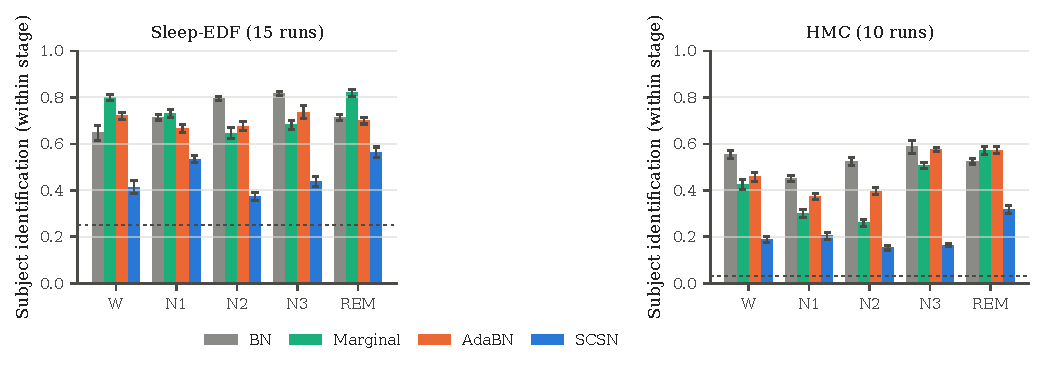
\includegraphics[width=\textwidth]{stage_identity}
\caption{Subject identification within each stage, mean over runs (Sleep-EDF:
fifteen runs; HMC: ten runs), for the uncorrected model (BN), the post-hoc
marginal correction, layerwise AdaBN and SCSN. Error bars are standard errors
over runs; the dashed line is chance. In two HMC runs a held-out recording
contributes fewer than five N3 epochs, so the N3 probe is undefined there;
the HMC N3 mean is over eight runs and the other HMC stages over ten. The
marginal correction moves the within-stage probe little on Sleep-EDF and
partway on HMC; SCSN reduces it in every stage.}
\label{fig:stage-identity}
\end{figure}

The accuracy result follows the same direction but is smaller. On Sleep-EDF
EEGNet SCSN changes accuracy by $+0.002$ [$-0.004$, $+0.009$], $p=0.36$, a
difference indistinguishable from zero; on HMC it gains $+0.019$ [$+0.010$,
$+0.028$], $p=0.0020$, over the uncorrected model, whereas the marginal
correction \emph{loses} $0.023$ [$-0.042$, $-0.005$], $p=0.010$. The HMC
pattern is the one the algebra predicts: marginal adaptation removes the
offset $a_{\cR}$ but adds the stage-mix residual
$\mu_{\mathrm{coh}}-\bar\mu_{\cR}$, which perturbs the logit margin, while
SCSN maps the conditional means back to the prototypes and restores the
margin. The Sleep-EDF cohort is smaller and more homogeneous, and the
accuracy effect there is not detectable.

\subsection{Layerwise AdaBN: what it removes and what it leaves}
\label{sec:adabn}

Layerwise AdaBN is the stronger marginal baseline: it re-estimates the
statistics of every normalization layer on the recording being scored and is
nonlinear. Under the matched probe protocol it changes the overall probe from
$0.715$ to $0.466$ and the within-stage probe from $0.738$ to $0.700$ on
Sleep-EDF EEGNet, and from $0.385$ to $0.212$ and $0.527$ to $0.473$ on HMC
EEGNet. It therefore removes part of the conditional signature as a side
effect, but less than SCSN: the paired difference in within-stage probe
between SCSN and AdaBN is $-0.235$ [$-0.266$, $-0.205$] on Sleep-EDF
($p<10^{-4}$) and $-0.264$ [$-0.278$, $-0.250$] on HMC ($p=0.0020$). On HMC
it also removes less than the post-hoc marginal correction, which moves the
probe from $0.527$ to $0.411$; layerwise statistics replacement is not a
monotone improvement on a single-vector correction.

Figure~\ref{fig:paired} shows the per-run paired structure behind these
averages: every run moves down from the uncorrected model to SCSN, and the
AdaBN points sit between the two.

\begin{figure}[t]
\centering
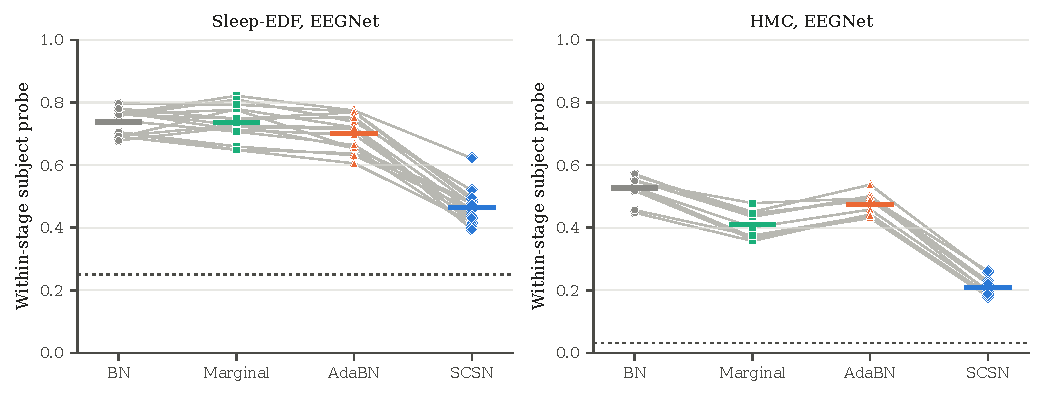
\includegraphics[width=\textwidth]{paired_probe}
\caption{Within-stage subject probe for every run (grey lines), with the arm
mean marked. Left: Sleep-EDF EEGNet, fifteen runs; right: HMC EEGNet, ten
runs. The uncorrected model, the marginal correction, layerwise AdaBN and
SCSN share the checkpoint and the probe subsample of each run.}
\label{fig:paired}
\end{figure}

The residual after AdaBN is informative about its nature. Applying SCSN to the
features produced by layerwise AdaBN changes the within-stage probe by
$-0.0004$ [$-0.0016$, $+0.0009$] ($p=0.85$), a difference that is not
distinguishable from zero: once
every layer has been adapted to the recording, what remains is not a
stage-conditional mean shift, and the correction that targets a mean shift has
nothing to remove. The two methods are therefore alternatives that remove
different components, not two stages of one pipeline. This is consistent with
the layerwise operation: re-estimating the statistics of a batch-normalized
layer rescales and recentres its output per recording, so any additively
stage-conditional component in that output is partly absorbed; what survives
is carried by the higher-order structure of the representation, which a
first-moment correction cannot reach.

\subsection{Accuracy, and where the methods separate}
\label{sec:accuracy}

SCSN is not the most accurate arm on every setting, and we report the
ordering rather than selecting the setting that favors it. On Sleep-EDF
EEGNet, the uncorrected model, the marginal correction, AdaBN and SCSN all
lie within $0.007$ of one another in accuracy, and the paired differences are
not significant (Table~\ref{tab:pairs}). On HMC EEGNet, SCSN is the most
accurate arm, $1.9$ points above the uncorrected model and $4.2$ points above
the marginal correction. On Sleep-EDF SleepCNN, layerwise AdaBN is more
accurate than SCSN by $0.014$ [$-0.033$, $+0.060$], a difference that is not
significant ($p=0.81$), and the uncorrected model is not significantly
different from SCSN. On HMC SleepCNN the three arms are closer: SCSN reaches
$0.712$ against $0.698$ for the uncorrected model and $0.702$ for AdaBN, a
significant gain over the former ($+0.014$ [$+0.006$, $+0.022$], $p=0.004$)
and a margin over the latter that is not significant ($+0.010$ [$-0.001$,
$+0.021$], $p=0.084$). The identity ordering is the
one that is stable across settings: SCSN has the lowest within-stage probe in
every one of the four batch-normalized settings, by margins between $0.27$ and
$0.44$ over the uncorrected model and between $0.24$ and $0.35$ over
layerwise AdaBN.

The Tent baseline is competitive on accuracy and does not remove the
stage-conditional identity. On Sleep-EDF EEGNet, SCSN reaches an accuracy of
$0.784$ against $0.782$ for Tent with the published optimizer on the same
fifteen runs, a difference of $+0.001$ [$-0.006$, $+0.008$], $p=0.85$, while
its within-stage probe is $0.465$ against $0.714$ for Tent, a difference of $-0.249$
[$-0.279$, $-0.220$], $p<10^{-4}$. On HMC EEGNet SCSN is $1.1$ points more
accurate ($+0.011$ [$+0.001$, $+0.021$], $p=0.037$) with a within-stage probe
of $0.209$ against $0.453$. On Sleep-EDF SleepCNN Tent is $1.8$ points more
accurate, a difference that is not significant ($p=0.44$), but its
within-stage probe is $0.858$ against $0.550$. Tent therefore keeps the patient
signature in every setting in which it was run. Tent optimizes a surrogate on the affine
parameters of the normalization layers; it is a batch-normalization method,
and adapting it requires a separate design for group-normalized checkpoints.
The comparison is therefore reported for the batch-normalized setting, and
the group-normalized experiment isolates the applicability of the proposed
correction.

\subsection{Class agreement, calibration and per-stage behavior}
\label{sec:agreement}

An accuracy gain could in principle come from predicting the most frequent
stage more often. The chance-corrected and class-balanced measures in
Tables~\ref{tab:main-eegnet} and~\ref{tab:main-sleepcnn} rule that out: Cohen's
$\kappa$ and the macro-averaged $F_1$ follow accuracy in every arm. Where SCSN
raises accuracy it raises both, by $0.023$ [$+0.012$, $+0.035$] in $\kappa$
and $0.018$ [$+0.008$, $+0.028$] in macro-$F_1$ on HMC EEGNet (paired
$p=0.002$ and $p=0.010$), and by $0.017$ [$+0.006$, $+0.027$] and $0.013$
[$+0.005$, $+0.020$] on HMC SleepCNN ($p=0.014$ and $p=0.006$). On Sleep-EDF the
differences are within noise: $\kappa$ changes by $+0.003$ ($p=0.36$) on
EEGNet and by $-0.005$ ($p=0.62$) on SleepCNN. The HMC gain is therefore
agreement across classes, not a reallocation toward the most frequent stage.

The per-stage recalls show where the accuracy difference comes from. On HMC,
the marginal correction buys N2 recall at the expense of wake and REM: on
EEGNet it raises N2 recall by $0.079$ ($p=0.002$) while lowering wake by
$0.107$ ($p=0.002$) and REM by $0.135$ ($p=0.014$), and on SleepCNN the same
pattern is $+0.063$ for N2 ($p=0.002$) against $-0.174$ for wake ($p=0.002$)
and $-0.036$ for N1 ($p=0.037$), with the losses in N3 and REM in the same
direction but not significant. The residual added by a single-vector correction is the
same for every epoch of the night, so it cannot be stage-specific; on these
checkpoints it shifts the decision toward N2, the most frequent stage. SCSN, which
removes the stage-conditional shift, raises N2 recall by $0.040$ ($p=0.006$)
on EEGNet and by $0.028$ ($p=0.006$) on SleepCNN without a significant loss
in any other stage. Its gain is an improvement of the decision boundary the
head was trained on, not a trade of one stage for another.

Calibration moves against accuracy on the small cohort. On Sleep-EDF EEGNet
SCSN raises the expected calibration error from $0.030$ to $0.044$ ($+0.013$
[$+0.006$, $+0.021$], $p=0.002$). The increase is not specific to SCSN ---
layerwise AdaBN reaches $0.043$ on the same runs --- but it is a cost of
correcting the representation, and it is the reason the limitation in
Section~\ref{sec:discussion} recommends recalibration. On HMC the change is
$+0.006$ ($p=0.049$) on EEGNet and $+0.002$ ($p=0.70$) on SleepCNN, and on the
group-normalized HMC EEGNet SCSN lowers the error by $0.009$ ($p=0.002$).
Conformal coverage is unaffected in every setting because the quantile is
refitted on the calibration split after the correction.

\subsection{Controls}
\label{sec:controls}

Table~\ref{tab:controls} reports the controls on the two EEGNet settings. The
interpolated family shows that identity removal is monotone in $\lambda$:
on Sleep-EDF the within-stage probe falls from $0.673$ at $\lambda=0.25$ to
$0.465$ at $\lambda=1$, while accuracy moves within $0.004$; on HMC it falls
from $0.434$ to $0.209$, while accuracy moves within $0.010$
(Figure~\ref{fig:interp}). The correction therefore buys identity without a
measurable accuracy trade-off on either cohort, and the endpoint $\lambda=0$
is the marginal correction whose within-stage probe is unchanged.

\begin{figure}[t]
\centering
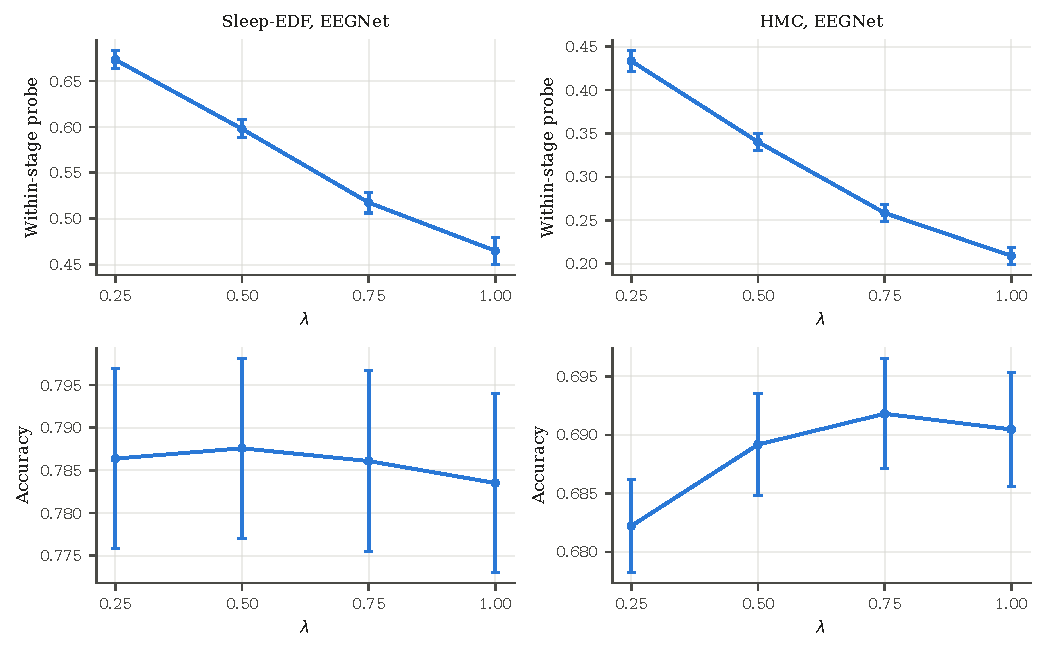
\includegraphics[width=0.85\textwidth]{interpolation}
\caption{The interpolated family: within-stage probe (top) and accuracy
(bottom) as a function of $\lambda$, for Sleep-EDF (left) and HMC (right).
$\lambda=1$ is SCSN, $\lambda\to0$ is the marginal correction. Identity
removal is monotone; accuracy is flat.}
\label{fig:interp}
\end{figure}

\begin{table}[t]
\centering
\caption{Controls on the batch-normalized EEGNet settings: mean accuracy,
within-stage probe, worst-patient conformal coverage and coverage dispersion
over fifteen runs (Sleep-EDF) and ten runs (HMC).}
\label{tab:controls}
\small
\resizebox{\columnwidth}{!}{\begin{tabular}{lrrrrrrrr}
\toprule
 & \multicolumn{4}{c}{Sleep-EDF, EEGNet} & \multicolumn{4}{c}{HMC, EEGNet} \\
\cmidrule(lr){2-5}\cmidrule(lr){6-9}
Arm & Acc & Within & Worst & SD & Acc & Within & Worst & SD \\
\midrule
BN & 0.781 & 0.738 & 0.828 & 0.055 & 0.672 & 0.527 & 0.649 & 0.086 \\
Marginal & 0.777 & 0.735 & 0.838 & 0.047 & 0.648 & 0.411 & 0.599 & 0.096 \\
SCSN-$\lambda_{0.25}$ & 0.786 & 0.673 & 0.837 & 0.049 & 0.682 & 0.434 & 0.665 & 0.079 \\
SCSN-$\lambda_{0.5}$ & 0.788 & 0.598 & 0.845 & 0.043 & 0.689 & 0.340 & 0.680 & 0.072 \\
SCSN-$\lambda_{0.75}$ & 0.786 & 0.518 & 0.851 & 0.039 & 0.692 & 0.258 & 0.678 & 0.069 \\
SCSN ($\lambda=1$) & 0.784 & 0.465 & 0.857 & 0.036 & 0.690 & 0.209 & 0.678 & 0.067 \\
SCSN-$r_1$ & 0.783 & 0.726 & 0.854 & 0.039 & 0.676 & 0.481 & 0.686 & 0.072 \\
SCSN-$r_2$ & 0.783 & 0.695 & 0.857 & 0.033 & 0.685 & 0.435 & 0.678 & 0.069 \\
SCSN-$r_4$ & 0.784 & 0.647 & 0.856 & 0.036 & 0.690 & 0.347 & 0.682 & 0.067 \\
SCSN-orth & 0.781 & 0.792 & 0.828 & 0.055 & 0.672 & 0.559 & 0.649 & 0.086 \\
SCSN-hard & 0.770 & 0.402 & 0.863 & 0.032 & 0.669 & 0.171 & 0.668 & 0.072 \\
SCSN-mismatch & 0.761 & 0.568 & 0.806 & 0.066 & 0.632 & 0.718 & 0.618 & 0.095 \\
\bottomrule
\end{tabular}
}
\end{table}

The rank restriction separates the two effects. Restricting the correction to
the top principal directions of the between-subject, within-stage covariance
removes much less identity than the full correction: $r=4$ leaves a
within-stage probe of $0.647$ on Sleep-EDF and $0.347$ on HMC, against
$0.465$ and $0.209$ for the full correction, and $r=1$ leaves $0.726$ and
$0.481$. Low rank does not buy accuracy: the full correction has the same
accuracy as $r=4$ on both cohorts ($p=0.93$ and $p=1.0$). The conditional
signature is therefore not confined to a few directions, and a practitioner
should not restrict the correction for efficiency.

The orthogonalised control projects each estimated shift off the row space of
the classifier, so the logits are unchanged exactly. Its accuracy is
identical to the uncorrected model on both cohorts, as it must be, and its
within-stage probe is \emph{higher} than the uncorrected model's
($0.792$ against $0.738$ on Sleep-EDF, $0.559$ against $0.527$ on HMC). The
projection removes the component of the shift that the classifier reads and
leaves the component it ignores, which is pure subject information; the
probe sees more of it. This is the clearest evidence that the identity change
in the SCSN arm is not a by-product of a change in predictions.

Two further controls bound the mechanism. Hard pseudo-labels over-correct:
they reduce the within-stage probe slightly more than the soft posterior
($0.402$ against $0.465$ on Sleep-EDF, $0.171$ against $0.209$ on HMC) but
cost $1.3$ and $2.2$ points of accuracy. Mismatched statistics --- applying
the shifts of another recording of the same fold --- remove less identity
($0.568$ and $0.718$ within-stage) and cost accuracy ($-0.022$ and $-0.059$
relative to SCSN, both significant). The effect therefore requires the
recording's own stage-conditional statistics, not merely a perturbation of the
representation.

The shrinkage constant $\lambda_s$ is the only hyperparameter of the
correction, and it is fixed at $10$ throughout. Re-running the SCSN arm with
$\lambda_s\in\{1,100\}$ on the same checkpoints and the same cached
representations, so that only the pseudo-count changes, shows where the value
matters. Between $\lambda_s=1$ and $10$ the arm moves by at most $0.001$ in
accuracy and $0.006$ in the within-stage probe on all four batch-normalized
settings. At $\lambda_s=100$ accuracy is again within $0.004$ points, but the
within-stage probe rises by $0.06$ to $0.11$: the pseudo-count now pulls the
estimated per-stage means towards the cohort prototypes, and the correction
removes less of the signature. The value used is therefore not tuned to the
reported result. Any pseudo-count between one and ten gives the same arm, and
the failure mode at a hundred is over-shrinkage, not sensitivity.

\subsection{Group-normalized stagers}
\label{sec:gn}

The group-normalized checkpoints are the setting in which standard AdaBN
cannot be applied because there is no test-time batch statistic. A bespoke
entropy objective on group-normalization affine parameters is a different
method and is not evaluated here. The post-hoc marginal correction applies,
and it removes the overall probe, but it moves
the within-stage probe by between a tenth and a third of what SCSN removes,
and not consistently in sign: on Sleep-EDF EEGNet it changes the within-stage
probe from $0.638$ to $0.616$ (paired $p=0.030$) and on Sleep-EDF SleepCNN
from $0.832$ to $0.889$, against $0.449$ and $0.583$ under SCSN (paired
changes of $-0.189$ [$-0.205$, $-0.174$] and $-0.248$ [$-0.284$, $-0.213$]).
On HMC EEGNet the uncorrected, marginal and SCSN within-stage probes are
$0.369$, $0.315$ and $0.156$, and on HMC SleepCNN they are $0.663$, $0.745$
and $0.341$; on the latter the marginal correction moves the probe in the
wrong direction (Figure~\ref{fig:gn}).

The accuracy effect points the same way and is smaller than on the
batch-normalized HMC model: SCSN gains $+0.010$ [$+0.005$, $+0.015$]
($p=0.003$) over the uncorrected group-normalized EEGNet and $+0.011$
[$+0.001$, $+0.022$] ($p=0.13$) over SleepCNN on Sleep-EDF, and $+0.016$
[$+0.013$, $+0.019$] and $+0.010$ [$+0.006$, $+0.014$] (both $p=0.0020$)
over HMC EEGNet and SleepCNN; on HMC SleepCNN the marginal correction
\emph{loses} two points. SCSN improves the worst-covered patient on the
Sleep-EDF checkpoints ($0.855$ to $0.864$ on EEGNet and $0.860$ to $0.870$ on
SleepCNN), although the marginal correction improves it there too. On HMC
EEGNet it improves the worst-covered patient from $0.695$ to $0.708$ and the
dispersion from $0.067$ to $0.059$, and on HMC SleepCNN from $0.677$ to
$0.697$ and from $0.070$ to $0.059$, although on both the marginal correction
improves the worst patient further ($0.724$).

\begin{figure}[t]
\centering
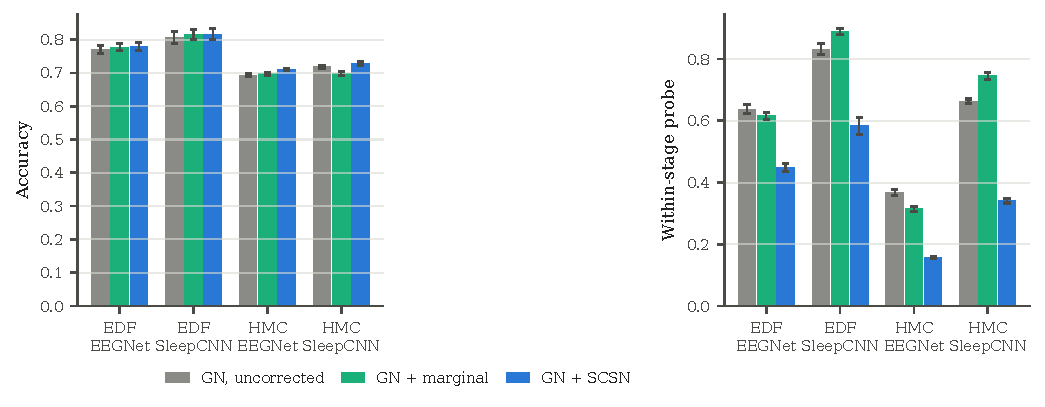
\includegraphics[width=\textwidth]{gn_arms}
\caption{Group-normalized checkpoints: accuracy (left) and within-stage
subject probe (right) for the uncorrected model, the post-hoc marginal
correction and SCSN. Error bars are standard errors over runs. The marginal
correction moves accuracy and the overall probe but barely moves the
within-stage probe; SCSN reduces it.}
\label{fig:gn}
\end{figure}

The result is the one the normalization argument predicts.
Group normalization removes the batch from the computation, so the
representation of an epoch depends only on that epoch; it does not follow
that the representation is free of the recording. The network that follows
the normalized layers maps the remaining recording-dependent variation into
the penultimate space, and a linear probe recovers the patient from it. Among
the statistics-replacement approaches compared here, SCSN is the only
stage-aware correction; it works without a batch statistic, optimizer, or
weight update.

\subsection{Patient-level conformal reliability}
\label{sec:coverage}

At $\alpha=0.1$ every arm covers at close to the nominal rate on average, and
the average hides the patient dependence. On Sleep-EDF EEGNet the
uncorrected model has a per-patient coverage standard deviation of $0.055$
and a worst-covered patient of $0.828$; the marginal correction improves them
to $0.047$ and $0.838$, and SCSN to $0.036$ and $0.857$. On HMC EEGNet the
same ordering holds against the uncorrected model: SCSN improves the
dispersion from $0.086$ to $0.067$ and the worst patient from $0.649$ to
$0.678$, while the marginal correction \emph{worsens} both ($0.096$ and
$0.599$). Layerwise AdaBN also improves the worst-covered patient over SCSN
in both settings ($0.866$ against $0.857$ on Sleep-EDF; $0.698$ against
$0.678$ on HMC), and its dispersion is smaller on Sleep-EDF ($0.028$ against
$0.036$) and comparable on HMC ($0.069$ against $0.067$). We report that
rather than the comparison that favors the method: on a batch-normalized
model, re-estimating every layer is a strong reliability intervention. On the
group-normalized checkpoints, where standard AdaBN is unavailable, SCSN
improves both quantities over the uncorrected model
(Table~\ref{tab:main-eegnet}).

Figure~\ref{fig:coverage} shows the empirical distribution of per-patient
coverage. Below the nominal level the uncorrected curve carries more mass
than the SCSN curve, and the marginal curve is the worst of the three on HMC;
above the nominal level the SCSN curve is the steeper one, so the shortfall of
the patients that do fall short is smaller. The review workload moves with the
sets: on Sleep-EDF EEGNet the fraction of multi-stage prediction sets falls
from $0.750$ to $0.729$ under SCSN and to $0.741$ under the marginal
correction.

\begin{figure}[t]
\centering
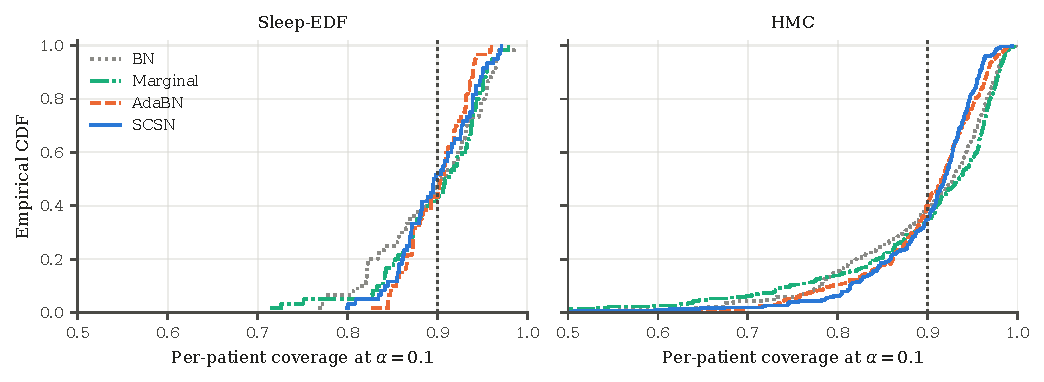
\includegraphics[width=\textwidth]{coverage_ecdf}
\caption{Empirical distribution of per-patient conformal coverage at
$\alpha=0.1$, pooled over runs. The dashed line is the nominal level. The
uncorrected model has more mass below the nominal level; the marginal
correction moves the distribution in the wrong direction on HMC, and SCSN
moves it in the right direction on both cohorts.}
\label{fig:coverage}
\end{figure}

\subsection{Transfer to a second centre, and the precondition of the method}
\label{sec:transfer}

A checkpoint trained on Sleep-EDF and never shown an HMC epoch is evaluated on
all $137{,}243$ HMC epochs under the source statistics, the post-hoc marginal
correction, SCSN, layerwise AdaBN and SCSN stacked on AdaBN
(Table~\ref{tab:cross}). This is a transfer across population, montage,
equipment, sampling rate and scoring manual, not merely across patients.

Under the source statistics the model reaches an accuracy of $0.475$ with a
worst-recording accuracy of $0.128$. The marginal correction raises accuracy
to $0.505$; layerwise AdaBN raises it to $0.553$ and the worst recording to
$0.214$. SCSN reaches $0.489$, below both. The oracle variant, which uses the
true stages to estimate the shifts, reaches $0.727$: the estimator is not the
limitation, the posterior is. When the source model is applied to a cohort it
was not trained on, its posterior is weak, the stage-conditional means
estimated from it are dominated by the prior and the recording offset, and the
correction behaves like the marginal one. SCSN should therefore not be applied
blindly across cohorts; the precondition is a posterior informative enough to
index the stages, and it can be checked on the unlabeled night before the
correction is applied.

\begin{table}[t]
\centering
\caption{Cross-cohort transfer: a Sleep-EDF checkpoint evaluated on all HMC
epochs. ``Worst'' and ``SD'' are the minimum and standard deviation of
per-recording accuracy. The group-normalized checkpoints have no statistics to
replace and are not part of this table.}
\label{tab:cross}
\small
\resizebox{\columnwidth}{!}{\begin{tabular}{lrrr}
\toprule
 & \multicolumn{3}{c}{EEGNet} \\
\cmidrule(lr){2-4}
 & Acc & Worst & SD \\
\midrule
Cohort statistics & 0.475 & 0.128 & 0.150 \\
Marginal & 0.505 & 0.115 & 0.143 \\
SCSN & 0.489 & 0.114 & 0.156 \\
SCSN-$\lambda_{0.5}$ & 0.497 & 0.113 & 0.152 \\
AdaBN & 0.553 & 0.214 & 0.134 \\
AdaBN + SCSN & 0.555 & 0.204 & 0.139 \\
SCSN (oracle labels) & 0.727 & 0.245 & 0.120 \\
\bottomrule
\end{tabular}
}
\end{table}

\begin{figure}[t]
\centering
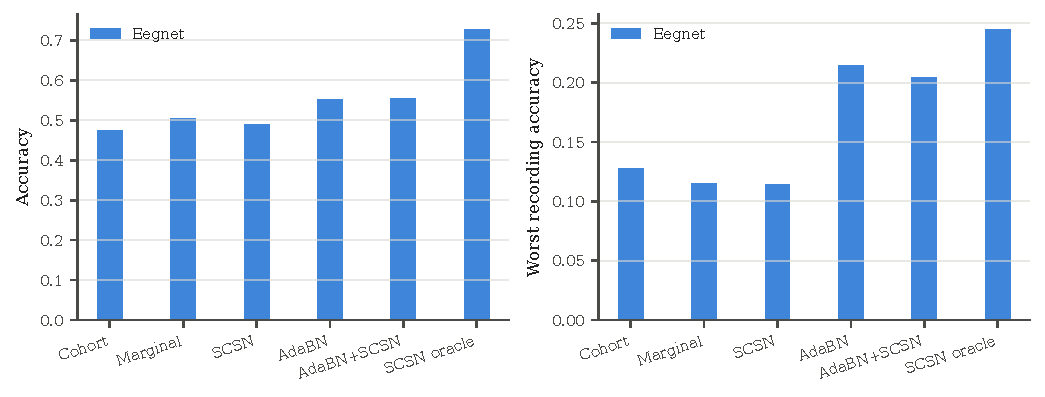
\includegraphics[width=\textwidth]{cross_cohort}
\caption{Cross-cohort accuracy (left) and worst-recording accuracy (right) for
the transferred checkpoint. The oracle uses the true stages; the gap between
it and SCSN is the cost of the weak target posterior.}
\label{fig:cross}
\end{figure}

Two caveats bound this experiment. Every arm is evaluated on a single
checkpoint, and no subject probe is computed on the transferred
representation, so the section speaks to accuracy and per-recording spread,
not to identity.
It shows that the intervention travels with the model to an unseen centre only
when the posterior does; the within-cohort experiments of
Sections~\ref{sec:scsn-identity}--\ref{sec:adabn} are what show that the
identity decomposition is the same there.

\section{Discussion}
\label{sec:discussion}

\subsection{What the decomposition buys}

The literature on subject variability in physiological signal classifiers is
mostly a literature about remedies: add a subject identifier, adversarially
remove one, fine-tune on the new patient. Each remedy is expensive in a
different currency --- annotations, training time, or a labeled target
cohort. The decomposition of Section~\ref{sec:method} separates the patient
into a recording-wide offset and a stage-conditional signature, and the
experiments show that the two parts have different remedies. The offset is
manufactured by the normalization layer and can be removed by replacing its
statistics, with no optimizer and no label. The signature can be targeted only
by an operation that knows the stage, and the inability of any marginal method
to target it is visible in the within-stage probe.

The decomposition also changes what a subject-invariance claim should report.
An overall probe conflates the two components: a single vector subtraction
per recording drives it close to chance even when the conditional signature
is untouched, because the recording mean is the dominant direction. A paper
that reports only the overall probe would conclude that marginal adaptation
and SCSN are equivalent on HMC --- both reach a probe near $0.07$ --- when
the within-stage probe is $0.41$ under the former and $0.21$ under the
latter. The within-stage probe is the quantity that matches the object the
classifier uses: the relative position of two stage-conditional means.

\subsection{Why marginal adaptation is not enough}

Proposition~\ref{prop:marginal} gives the residual of any correction that
subtracts one vector per recording: $\mu_k+s_{\cR,k}+(\mu_{\mathrm{coh}}-\bar
\mu_{\cR})$. The first two terms say that the class-conditional means are
still those of the patient, not those of the cohort; the third says that the
correction adds an offset determined by the patient's stage mix. The second
term is why the within-stage probe survives. The third is why marginal
adaptation can \emph{lose} accuracy: on HMC, where recordings differ in stage
mix and the cohort is large, the post-hoc marginal arm is $2.3$ points worse
than the uncorrected model. The loss is not spread evenly over the night: on
HMC EEGNet the marginal arm gives up $0.135$ of REM recall and $0.107$ of
wake recall for $0.079$ of N2 recall, whereas SCSN raises N2 recall by
$0.040$ without a significant loss in any stage
(Section~\ref{sec:agreement}). An oracle marginal correction that knew the
recording's stage mix would remove the third term but not the second; the
signature is out of reach of any operation that uses one mean per recording.

SCSN removes both terms with the model's own posterior. The price is that the
posterior must be informative: the residual of the soft correction is the part
of the signature assigned to the wrong stage, bounded by the posterior error.
The cross-cohort experiment is the regime in which that price is not paid, and
the degradation there is the clearest evidence that the mechanism is the one
the algebra describes rather than an unspecified regularisation effect.

\subsection{What kind of claim this is}

The method can be read as an inference-time trick, and that reading would miss
what is being claimed. Nothing here changes the training procedure, the
architecture or the objective; the operation is arithmetic on a frozen
representation, and it is not presented as a new architecture or a new learning
objective. The claim is nevertheless about the model: that the
stage-conditional means of its penultimate representation are shifted by the
patient, that the shift is identifiable from the recording and the model's own
posterior, and that no operation using a single vector per recording can
remove it (Corollary~\ref{cor:no-marginal}). That is a statement about what the network
has learned, in the same sense as a probing result, and the paper makes it
falsifiable with a measurement it introduces: the within-stage probe falls
under SCSN and does not fall under any marginal correction, in every setting
tested. The estimator then follows from the statement through the conditional
expectation of the shift given the model's posterior
(Remark~\ref{rem:mmse}), and the closed form follows from the deployment
setting in which such a statement is useful: a checkpoint whose weights are
frozen and a night whose labels are unknown. A method that needed a second
pass, an optimizer or a gradient through the posterior would answer the same
analytical question and be a different engineering object. The object of the
contribution is the analysis and the measurement. The algorithm is what that
analysis leaves as the only available operation; its deployment properties are
what make the analysis usable at the bedside, and they are not where the
novelty lies.

\subsection{When the correction is free and when it is not}

On Sleep-EDF EEGNet, SCSN leaves accuracy where the uncorrected model and
layerwise AdaBN leave it; on HMC EEGNet and HMC SleepCNN it gains $1.9$ and
$1.4$ points over the uncorrected model and has the highest mean accuracy of
the arms, although on HMC SleepCNN the margin over layerwise AdaBN is not
significant ($p=0.084$).
The HMC gains survive the chance-corrected and class-balanced measures:
$\kappa$ rises by $0.023$ and $0.017$ and macro-$F_1$ by $0.018$ and $0.013$
on the two backbones, with no comparable change on Sleep-EDF.
On Sleep-EDF SleepCNN, layerwise AdaBN is $1.4$ points more accurate than
SCSN, a difference that is not significant. We report the ordering rather
than selecting the cohort on which the method wins. Two mechanisms plausibly
explain the ordering. Layerwise AdaBN is nonlinear and acts at every layer:
it removes part of the conditional signature as a side effect, lowering the
within-stage probe by $0.04$ to $0.09$ where it acts at all, and not at all
on Sleep-EDF SleepCNN, but it has no stage index and cannot target that
signature; SCSN removes $0.24$ to $0.35$ more. And the accuracy effect of
SCSN depends on the posterior: where the posterior is weak, the correction
approaches the marginal one, as the cross-cohort experiment shows. Neither
mechanism makes SCSN preferable on accuracy alone on Sleep-EDF; the case for
SCSN there rests on the identity it removes and on the fact that the same
operation is the only one available on a group-normalized checkpoint.

Tent is a strong baseline on Sleep-EDF and we do not claim to beat it on
accuracy. It is also a batch-normalization method: it optimizes the affine
parameters of batch-normalization layers. Applying it unchanged to a
group-normalized model is not defined, and a GroupNorm-specific entropy method
would require a separate design and tuning protocol. The comparison is
therefore reported for the batch-normalized checkpoints where both methods are
defined.

\subsection{The group-normalized setting}

Group normalization is often described as removing subject information
because it removes the batch. The experiments show that it does not remove
the patient: a linear probe identifies the patient from a group-normalized
representation well above chance on both cohorts and both backbones. What it
removes is the batch dependence of the normalization, not the
recording-dependent variation that the following layers map into the
penultimate space.

This is the setting in which the contribution is least ambiguous within the
family considered here. Standard AdaBN is undefined because there is no
test-time batch statistic, and standard Tent targets batch-normalization
affine parameters. The post-hoc marginal correction is defined and removes
the overall probe, but it moves the
within-stage probe by between a tenth and a third of what SCSN removes, and
in the wrong direction on both SleepCNN checkpoints, because a single vector
per recording carries no stage index. SCSN is the only stage-aware
statistics-replacement correction among those evaluated, and on the
group-normalized checkpoints it improves accuracy and the worst-covered
patient over the uncorrected model. A practitioner who chooses group
normalization for its batch independence therefore has a label-free
inference-time correction available without changing the architecture.

\subsection{Reading the reliability result correctly}

The conformal guarantee is marginal over patients, and the numbers make the
sense in which it is marginal concrete: every arm covers at about the nominal
rate on average, while the worst-covered patient of a fold is covered well
below it. The dispersion of per-patient coverage is the quantity that
separates a model whose guarantee is uniform from one whose guarantee is an
average.

The correction that removes the patient signature also reduces the
concentration of failures, but not uniformly across settings. On the
group-normalized checkpoints SCSN improves the worst-covered patient and the
dispersion in all four settings. On
the batch-normalized EEGNet checkpoints, layerwise AdaBN attains a better
worst-covered patient than SCSN ($0.866$ against $0.857$ on Sleep-EDF and
$0.698$ against $0.678$ on HMC) and a smaller dispersion on Sleep-EDF ($0.028$
against $0.036$), with the two dispersions comparable on HMC ($0.069$ against
$0.067$); on HMC SleepCNN the ordering reverses, with SCSN better on both
quantities ($0.664$ against $0.649$ and $0.066$ against $0.072$). We report
that rather than the comparison that favors the method. The safe statement is the mechanistic one: removing the
component of the representation that carries the patient reduces the
patient-dependence of the coverage, and the size of the reduction depends on
how much of that component the correction removes.

\subsection{The boundary of the method}

The cross-cohort experiment defines the regime in which a stage-conditional
correction should not be used. When a model trained on one centre is applied
to another, its posterior is weak, and the stage-conditional means estimated
from that posterior are dominated by the prior and by the recording offset.
SCSN then performs like the marginal correction and below layerwise AdaBN; the
oracle-label version, which uses the true stages to estimate the shifts,
recovers a large part of the gap, so the limitation is the posterior rather
than the estimator. This is a useful diagnostic: the method has a measurable
precondition, and the precondition can be checked on the unlabeled night
before the correction is applied, for example by the entropy or the
confidence of the uncorrected posterior.

\subsection{Limitations}

\paragraph{Cohort size}
Sleep-EDF has 20 subjects, so a fold holds out four of them and the probe is a
four-way problem. A four-way probe can only be so informative, and a
subject-level statistic computed over four subjects is noisy. This is the
reason the paper carries a second cohort of 151 subjects; the second cohort is
larger than most in the literature but comes from one centre, one montage and
one scoring team, and it is a cohort of patients referred for suspected sleep
disorders rather than of healthy volunteers.

\paragraph{Probe capacity}
The probe is a linear readout. A nonlinear probe would find more identity in
every arm, and the fractions reported here are lower bounds on what the
representation contains rather than statements about what it contains. The
comparison between arms is not affected by this, since the probe is the same
object in every arm, but the absolute level should be read as a floor.

\paragraph{Backbones}
Two convolutional backbones are used on both cohorts, chosen to differ in
depth, width and receptive field. Neither is a transformer, and the extent to
which normalization-driven identity matters in attention-based stagers is not
addressed here.

\paragraph{Posterior quality}
The correction is only as good as the posterior that indexes the stages. On
the within-cohort experiments the posterior is informative enough that the
correction is close to exact; across cohorts it is not, and the method
degrades to the marginal correction. A stager with a poorly calibrated head
would need the head recalibrated before the correction is applied.

\paragraph{Probability calibration}
Re-estimating the statistics, or correcting the representation, changes the
scale of the logits relative to the scale on which the posterior head was
fitted, and the expected calibration error moves with it: on Sleep-EDF EEGNet
from $0.030$ to $0.044$, with layerwise AdaBN at $0.043$ on the same runs, and
by at most $0.006$ on HMC. Conformal sets are
unaffected in coverage because their quantile is refitted on the calibration
split after the same intervention, but a user who reads the raw probabilities
of a deployed stager should recalibrate them after the correction.

\paragraph{Offline operation}
As with AdaBN, the statistics are estimated on the whole night. Clinical
staging is scored after the night, so the constraint is not binding in the
application we target, but a real-time monitor would have to estimate the
statistics on a prefix, which we have not tested.

\paragraph{GroupNorm-specific test-time adaptation}
Because group normalization has learnable affine parameters, an entropy-based
test-time objective could be designed for it. We did not implement that
baseline here: doing so would introduce a new optimizer, step-size schedule,
and stopping rule, and would no longer be the standard Tent method. The
group-normalized comparison therefore establishes applicability and internal
mechanism, not superiority to every possible GroupNorm-specific adaptation
objective.

\paragraph{Single channel}
Both cohorts are staged from a single EEG derivation. Multi-channel stagers
have more ways to encode a patient, and the balance between the marginal and
the conditional part of the identity may differ.

\paragraph{Statistical inference}
The Wilcoxon tests are exploratory and pairwise unadjusted. Seeds within a
fold reuse the same held-out subjects, so paired runs are not fully
independent; fold-level sign counts are therefore reported alongside the
run-level tests to reduce reliance on pseudo-replication. We make no
familywise-error claim. The consistency of effect directions across cohorts,
backbones, and normalization schemes, rather than any single $p$-value, is
the basis for the conclusions.

\subsection{Practical recipe}

For a stager that is already trained and validated, the procedure the results
support is short.
\begin{enumerate}
  \item Fit a linear probe from the penultimate representation to the patient,
  overall and within stage. If the overall probe is near chance, the marginal
  patient is not in the representation. If the within-stage probe is near
  chance, the conditional signature is not there either, and no
  stage-conditional correction is needed.
  \item If the within-stage probe is high, apply SCSN on each recording before
  predicting it. On a batch-normalized model, compare with layerwise AdaBN; on
  a group-normalized model, SCSN is the only stage-conditional option.
  \item Check the uncorrected posterior before applying the correction. If it
  is close to uniform, the stage-conditional means are not identifiable and
  the correction should be reduced to the marginal one.
  \item Recalibrate the conformal score on recordings processed the same way,
  and report per-patient coverage dispersion beside average coverage.
\end{enumerate}
The first step is a diagnostic that costs one logistic regression; the second
adds a few matrix products to the forward pass the stager performs anyway; the
third is a scalar check on the posterior; the fourth is bookkeeping. None of them requires a labeled target cohort, and
all of them can be applied to a model whose weights will never be touched
again.

\section{Conclusion}
\label{sec:conclusion}

A stager's representation of a patient has two parts. One is a recording-wide
offset manufactured by the normalization statistics; the other is a
stage-conditional signature that describes how this patient's sleep stages
differ from the cohort prototypes. Marginal adaptation removes the first and,
as the within-stage probe shows, cannot target the second. Layerwise
adaptation may absorb part of it as a nonlinear side effect, but a
stage-conditional operation is required to remove the signature explicitly.
Stage-conditional shift normalization removes it with the model's own
posterior, in closed form, at the cost of one pass over the unlabeled night.

The experiments support three statements. The within-stage probe separates the
two components where the overall probe cannot, and it is the measurement a
subject-invariance claim should report. SCSN reduces that probe in every
setting, by between $0.19$ and $0.44$, and on the group-normalized checkpoints
it is the only stage-aware statistics-replacement method evaluated that does
so. Where it changes accuracy, it improves
it: significantly on the HMC backbones and on three of four group-normalized
settings, not measurably on Sleep-EDF EEGNet, and within noise of layerwise
AdaBN on both SleepCNN settings; the gains survive chance correction and class
balancing, and they come with a better worst-covered patient and a smaller
coverage dispersion.

The limitations define the next experiments. The method is evaluated on two
single-channel convolutional backbones, its estimate is only as good as the
posterior that indexes the stages, and it assumes the whole night is available.
A multi-channel or attention-based stager, a recalibrated posterior, and a
prefix-based online variant are the natural places to test whether the
decomposition --- rather than the particular estimator --- is what carries the
result.


\section*{Declaration of competing interest}
The authors declare that they have no known competing financial interests or
personal relationships that could have appeared to influence the work
reported in this paper.

\section*{Funding}
This research did not receive any specific grant from funding agencies in the
public, commercial, or not-for-profit sectors.

\section*{Data availability}
Sleep-EDF and the Haaglanden Medisch Centrum Sleep Staging Database are
publicly available from PhysioNet at
\url{https://physionet.org/content/sleep-edfx/1.0.0/} and
\url{https://physionet.org/content/hmc-sleep-staging/1.1.0/}, respectively.

\section*{Code availability}
The code that produces every number and figure of this paper, together with
the trained-checkpoint evaluation scripts and released result summaries, is
available at \url{https://github.com/YuhaoPeng1103/SleepSCSN}.

\section*{Ethics statement}
This study used publicly available, de-identified Sleep-EDF and HMC recordings
from PhysioNet. No new human-subject data were collected, and additional
ethics approval was therefore not required.

\section*{CRediT authorship contribution statement}
\textbf{Zhiwen Song:} Conceptualization, Methodology, Software, Validation,
Formal analysis, Investigation, Writing -- original draft. \textbf{Yuhao
Peng:} Supervision, Writing -- review \& editing.

\section*{Declaration of generative AI and AI-assisted technologies}
During the preparation of this work, the authors used OpenAI Codex to assist
with language editing, manuscript organization, and consistency checks. The
authors reviewed and edited the content as needed and take full responsibility
for the content of the publication.

\bibliography{refs}

\end{document}
